\documentclass[10pt,letterpaper]{article}
\usepackage[utf8]{inputenc}
\usepackage[T1]{fontenc}
\usepackage[margin=0.6in]{geometry}
\usepackage{amsmath,amssymb,mathtools,graphicx,booktabs,xcolor,hyperref}
\setlength{\parindent}{0pt}
\setlength{\parskip}{5pt}
\begin{document}

{\color{ink}\sffamily\bfseries\LARGE Block S1: Equivalent Resistance \& Multi-Source KVL/KCL}\par
\textbf{Study Window:} Sunday 2:45--3:50 PM (65 min) \quad|\quad \textbf{Source Grounding:} Young \& Freedman 13e Ch.\ 25--26 (\texttt{yf13-review-block-s1-v1})

\section*{Exercise 01 $\cdot$ First-Principles \& Calculus Derivations \hfill [10 Points $\cdot$ DERIVE]}
\begin{enumerate}
  \item[(a)] \textbf{Series Equivalence from KVL [2 pts]:} Consider $N$ resistors $R_1, R_2, \dots, R_N$ connected in series across terminal voltage $V_{ab}$. Using steady-state charge conservation ($\nabla\cdot\mathbf{J}=0$) and Kirchhoff's loop rule ($\sum_{\rm loop}\Delta V = 0$, including the source rise), prove that $R_{\text{eq}} = \sum_{k=1}^{N} R_k$.
  \item[(b)] \textbf{Parallel Equivalence from KCL [2 pts]:} Consider $N\ge 2$ positive resistors connected in parallel between nodes $a$ and $b$. Using Kirchhoff's junction rule ($\sum I_{\text{in}} = \sum I_{\text{out}}$) and common node potentials, prove that $\frac{1}{R_{\text{eq}}} = \sum_{k=1}^{N} \frac{1}{R_k}$, and prove algebraically that $R_{\text{eq}} < \min_k(R_k)$.
  \item[(c)] \textbf{Continuous Non-Uniform Conductor (``Problem with Calculus'') [6 pts]:} A conductor of length $L$ and uniform resistivity $\rho$ has the shape of a truncated right circular cone (frustum) whose radius varies from $a$ at $x = 0$ to $b$ at $x = L$. Use the idealized one-dimensional slice model: treat each cross-section as equipotential and neglect spreading and edge effects, so the same current $I$ passes through each disk slice.
  \begin{center}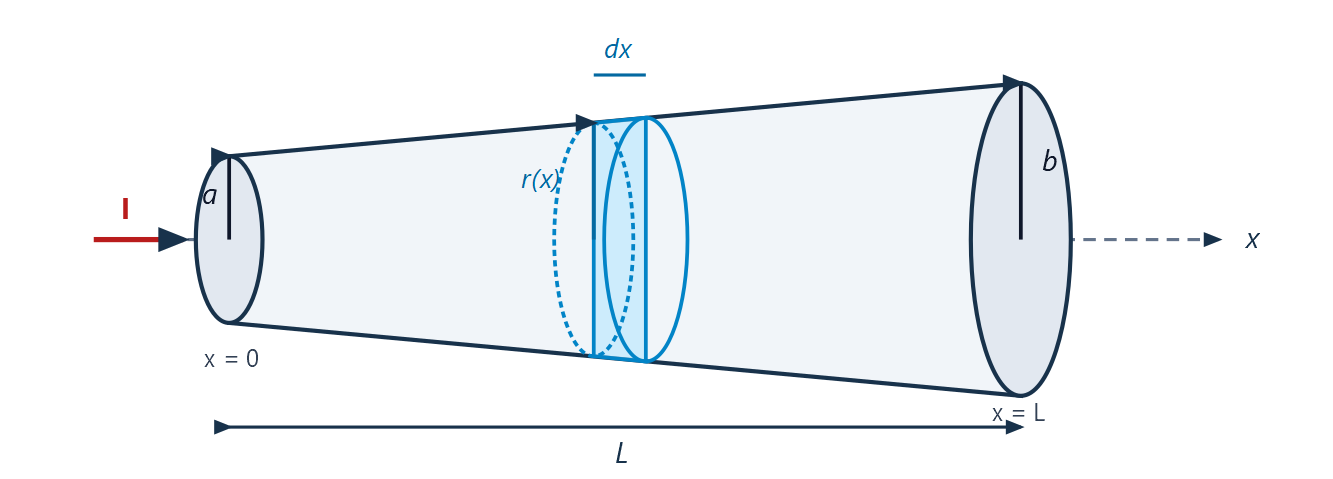
\includegraphics[width=0.72\linewidth]{block_s1_assets/s1-q1-cone.png}\end{center}
  \begin{enumerate}
    \item[(i)] Write the cross-sectional radius $r(x)$ and area $A(x)$ at axial position $x \in [0, L]$, and write the differential resistance $dR$ of an infinitesimal disk slab of thickness $dx$.
    \item[(ii)] Integrate $R_{\rm 1D} = \int_0^L dR$ explicitly to find the resistance predicted by this slice model.
    \item[(iii)] Verify that your formula recovers the elementary uniform-cylinder formula in the limit $b \to a$, and find the electric field magnitude $E(x)$ as a function of $x$ in terms of $I, \rho, a, b, L$.
  \end{enumerate}
\end{enumerate}

\newpage
\section*{Exercise 02 $\cdot$ Mixed Series--Parallel DC Ladder \& Short-Circuit Perturbation \hfill [10 Points $\cdot$ FR]}
An ideal DC voltage source $V_s = 36.0\text{ V}$ supplies a series resistor $R_1 = 6.00\ \Omega$ connected at junction $B$ to two parallel branches: branch 1 contains $R_2 = 18.0\ \Omega$ alone, and branch 2 contains $R_3 = 4.00\ \Omega$ in series with $R_4 = 5.00\ \Omega$. Node $G$ is grounded ($V_G = 0\text{ V}$).
\begin{center}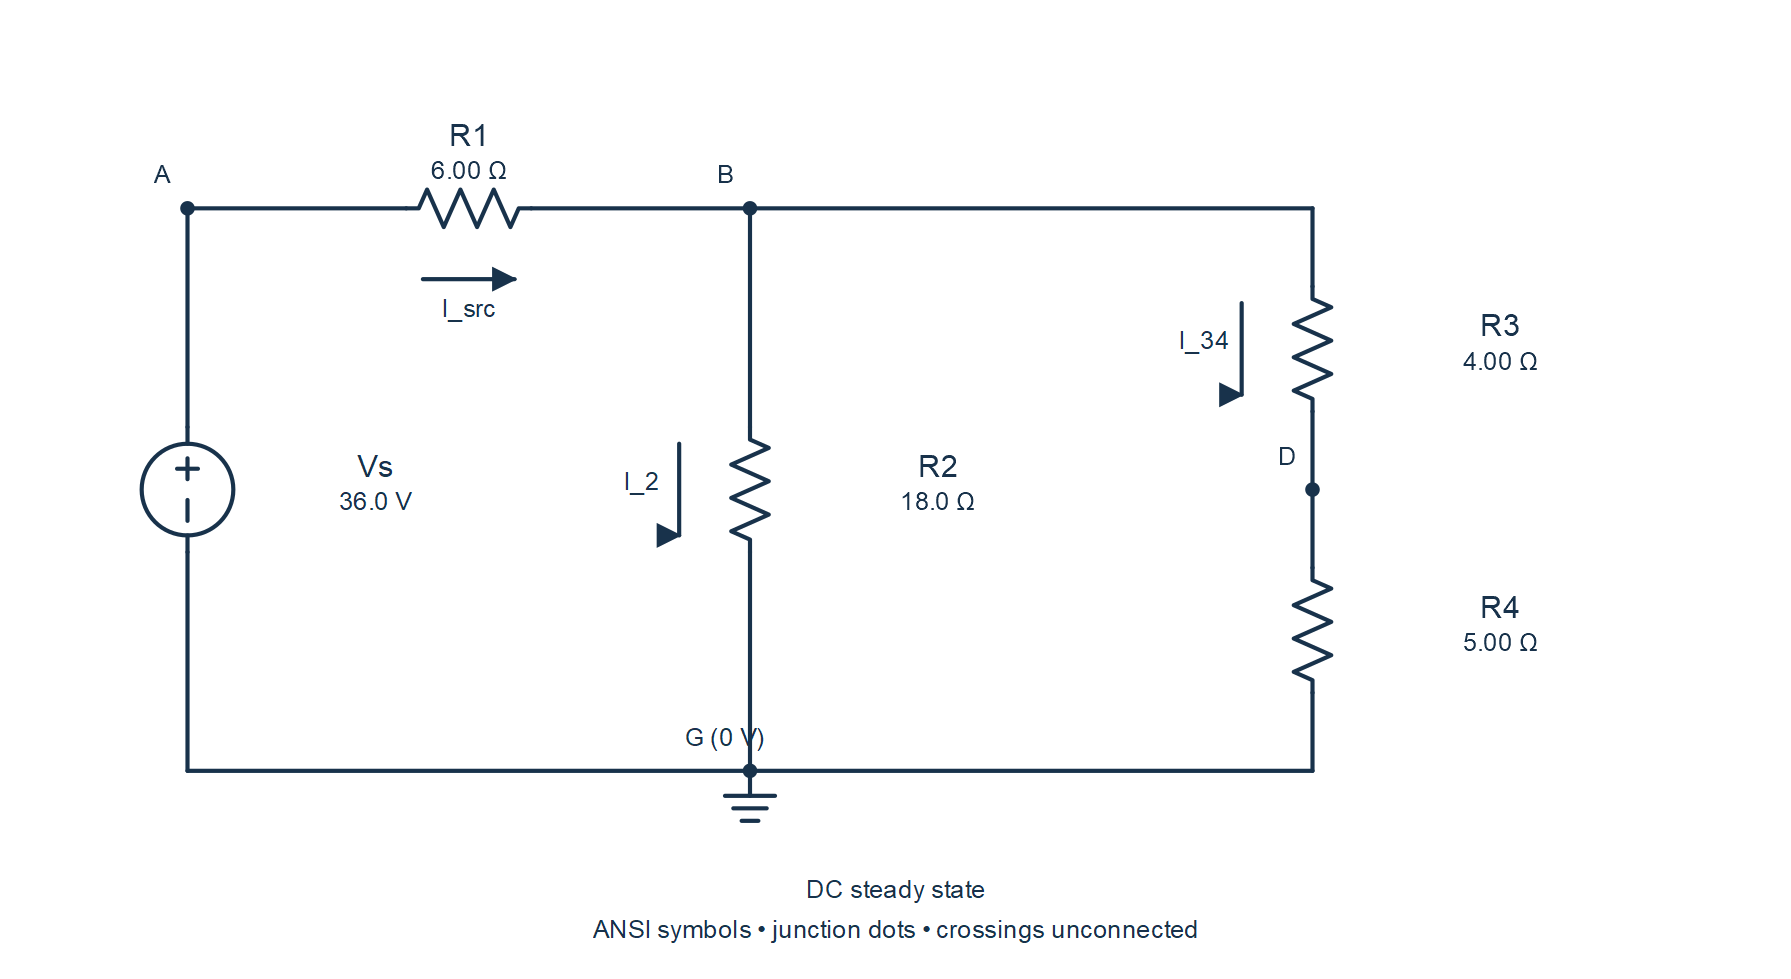
\includegraphics[width=0.75\linewidth]{block_s1_assets/s1-q2-ladder.png}\end{center}
\begin{enumerate}
  \item[(a)] \textbf{Network Reduction [2 pts]:} Calculate the equivalent resistance $R_{BG}$ of the parallel block between node $B$ and ground $G$, and the total equivalent resistance $R_{\text{eq}}$ seen by the $36.0\text{ V}$ source.
  \item[(b)] \textbf{Branch Currents \& Node Potentials [3 pts]:} Determine the source current $I_{\text{src}}$, the node potentials $V_B$ and $V_D$, and the branch currents $I_2$ and $I_{34}$. Verify that $I_2$ and $I_{34}$ satisfy both KCL at node $B$ and the current-divider ratio.
  \item[(c)] \textbf{Power Bookkeeping [2 pts]:} Compute the electrical power dissipated in each of the four resistors ($P_{R_1}, P_{R_2}, P_{R_3}, P_{R_4}$) and verify that $\sum_{k=1}^4 P_{R_k} = P_{\text{source}} = V_s I_{\text{src}}$.
  \item[(d)] \textbf{Topology Perturbation (Shorted Element) [3 pts]:} Suppose a metallic jumper wire accidentally shorts node $B$ directly to node $D$ (so $R_3$ is bypassed, $R_3 \to 0$). Calculate the new equivalent resistance $R_{\text{eq}}'$, the new source current $I_{\text{src}}'$, and the new power $P_{R_4}'$ dissipated in $R_4$. By what factor does $P_{R_4}$ increase?
\end{enumerate}

\newpage
\section*{Exercise 03 $\cdot$ Multi-Source KVL/KCL Network \& Power Direction \hfill [12 Points $\cdot$ FR]}
Three parallel branches connect top junction $A$ to grounded bottom reference node $B$ ($V_B = 0\text{ V}$). Each ideal EMF source has its positive ($+$) terminal oriented upward. Downward reference currents $I_1, I_2, I_3$ are defined from node $A$ toward node $B$ as shown in the Spec v2 schematic below.
\begin{center}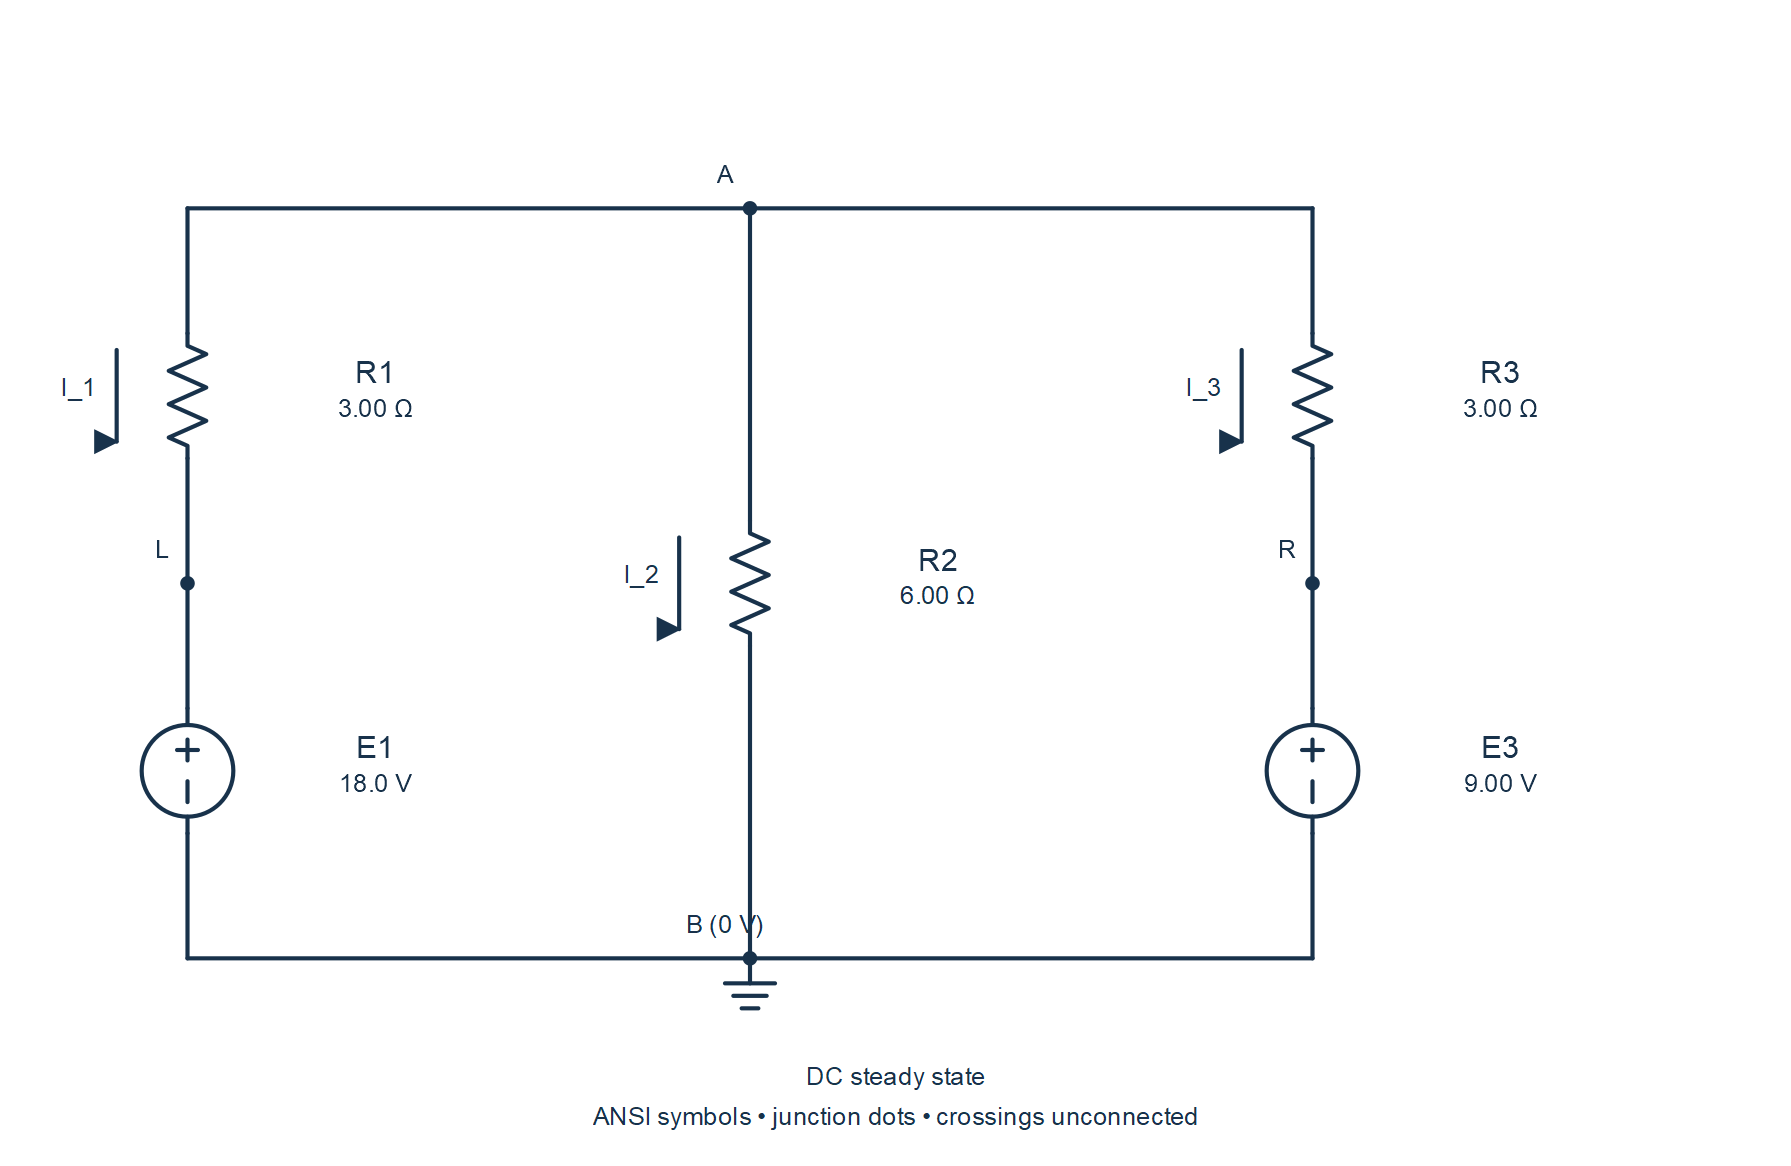
\includegraphics[width=0.76\linewidth]{block_s1_assets/s1-q3-multisource.png}\end{center}
\begin{enumerate}
  \item[(a)] \textbf{KCL \& KVL Formulation [3 pts]:} Write (i) the KCL junction equation at node $A$ in terms of $I_1, I_2, I_3$, (ii) the KVL loop equation around the left mesh (containing $\mathcal{E}_1, R_1, R_2$), and (iii) the KVL loop equation around the right mesh (containing $R_2, R_3, \mathcal{E}_3$).
  \item[(b)] \textbf{Nodal \& Mesh Solution [5 pts]:} Express $I_1, I_2, I_3$ in terms of the single unknown node potential $V_A$, solve for $V_A$, and compute the signed currents $I_1, I_2, I_3$. State the actual physical direction (upward or downward) of current in each branch, and verify that your currents satisfy both KVL equations from part (a).
  \item[(c)] \textbf{Source Power Delivery vs.\ Absorption [4 pts]:} For each EMF source ($\mathcal{E}_1 = 18.0\text{ V}$ and $\mathcal{E}_3 = 9.00\text{ V}$), determine whether the source is \textbf{delivering} electrical power to the circuit or \textbf{absorbing} electrical power (being charged). Calculate both source powers and verify global conservation of energy against total resistor Joule heating $\sum_{k=1}^3 I_k^2 R_k$.
\end{enumerate}

\newpage
\section*{Exercise 04 $\cdot$ Conceptual Cloze \& Maximum Power Transfer Graphs \hfill [10 Points $\cdot$ CLOZE + DRAW]}
\subsection*{Part A: Conceptual Cloze with Word Bank [4 points --- 0.5 pt each]}
\noindent\colorbox{pale}{\parbox{\dimexpr\linewidth-2\fboxsep\relax}{%
\textbf{WORD BANK:} \texttt{electric charge} $\cdot$ \texttt{energy} $\cdot$ \texttt{magnetic flux} $\cdot$ \texttt{smaller than} $\cdot$ \texttt{larger than} $\cdot$ \texttt{opposite to} $\cdot$ \texttt{equal to} $\cdot$ \texttt{$\mathcal{E} - Ir$} $\cdot$ \texttt{$\mathcal{E} + Ir$} $\cdot$ \texttt{open circuit} $\cdot$ \texttt{short circuit} $\cdot$ \texttt{zero}%
}}
\begin{enumerate}
  \item[(a)] Kirchhoff's junction rule (KCL, $\sum I = 0$) is a direct statement of local conservation of \underline{\hspace{2.2in}} at a steady-state node.
  \item[(b)] Kirchhoff's loop rule (KVL, $\sum_{\rm loop} \Delta V = 0$, including source rises and resistor drops) follows from conservation of \underline{\hspace{2.2in}} per unit charge.
  \item[(c)] When any positive resistor $R_{\text{new}}$ is connected in parallel across an existing resistor network, the new equivalent resistance is strictly \underline{\hspace{2.2in}} the smallest individual branch resistance.
  \item[(d)] If solving a KVL/KCL system yields $I_1 = -2.40\text{ A}$, the negative sign means the actual current has magnitude $2.40\text{ A}$ and flows \underline{\hspace{2.2in}} the assumed reference arrow.
  \item[(e)] When a real battery (EMF $\mathcal{E}$, internal resistance $r$) supplies current $I$ out of its positive terminal (discharging), its terminal voltage is \underline{\hspace{2.2in}}.
  \item[(f)] When an external source forces current $I$ \emph{into} the positive terminal of a real battery (charging), its terminal voltage is \underline{\hspace{2.2in}}.
  \item[(g)] An ideal voltmeter has infinite internal resistance and behaves as an \underline{\hspace{2.2in}} when connected in parallel across a circuit element.
  \item[(h)] An ideal ammeter has negligible resistance and behaves like a \underline{\hspace{2.2in}} when inserted in series.
\end{enumerate}

\subsection*{Part B: Draw the Effect \& Calculus of Maximum Power Transfer [6 points --- DRAW + DERIVE]}
A real DC source has open-circuit EMF $\mathcal{E} = 18.0\text{ V}$ and internal resistance $r = 3.00\ \Omega$, and is connected across a variable load resistor $R_L \in [0, 15.0\ \Omega]$.
\begin{enumerate}
  \item[(i)] \textbf{Calculus Proof [2 pts]:} Express $P_L(R_L)=I^2R_L$ in terms of $\mathcal{E}$, $r$, and $R_L$. Differentiate, find and classify the stationary point, then calculate its resistance and peak power.
  \item[(ii)] \textbf{Plot 1 [2 pts]:} On grid (i) below, plot the terminal voltage $V_T$ (\textbf{dependent variable}, vertical axis, in $\text{V}$) vs.\ load current $I$ (\textbf{independent variable}, horizontal axis, in $\text{A}$) from $I = 0$ to $I_{\text{sc}} = 6.00\text{ A}$. Label the open-circuit intercept, the short-circuit intercept, the operating point at $R_L = r$, and the slope.
  \item[(iii)] \textbf{Plot 2 [2 pts]:} On grid (ii) below, plot the load power $P_L$ (\textbf{dependent variable}, vertical axis, in $\text{W}$) vs.\ load resistance $R_L$ (\textbf{independent variable}, horizontal axis, in $\Omega$) for $0 \le R_L \le 15.0\ \Omega$. Mark the peak found in (i) and label the values at $R_L=0$, $6.00\ \Omega$, and $15.0\ \Omega$.
\end{enumerate}
\begin{center}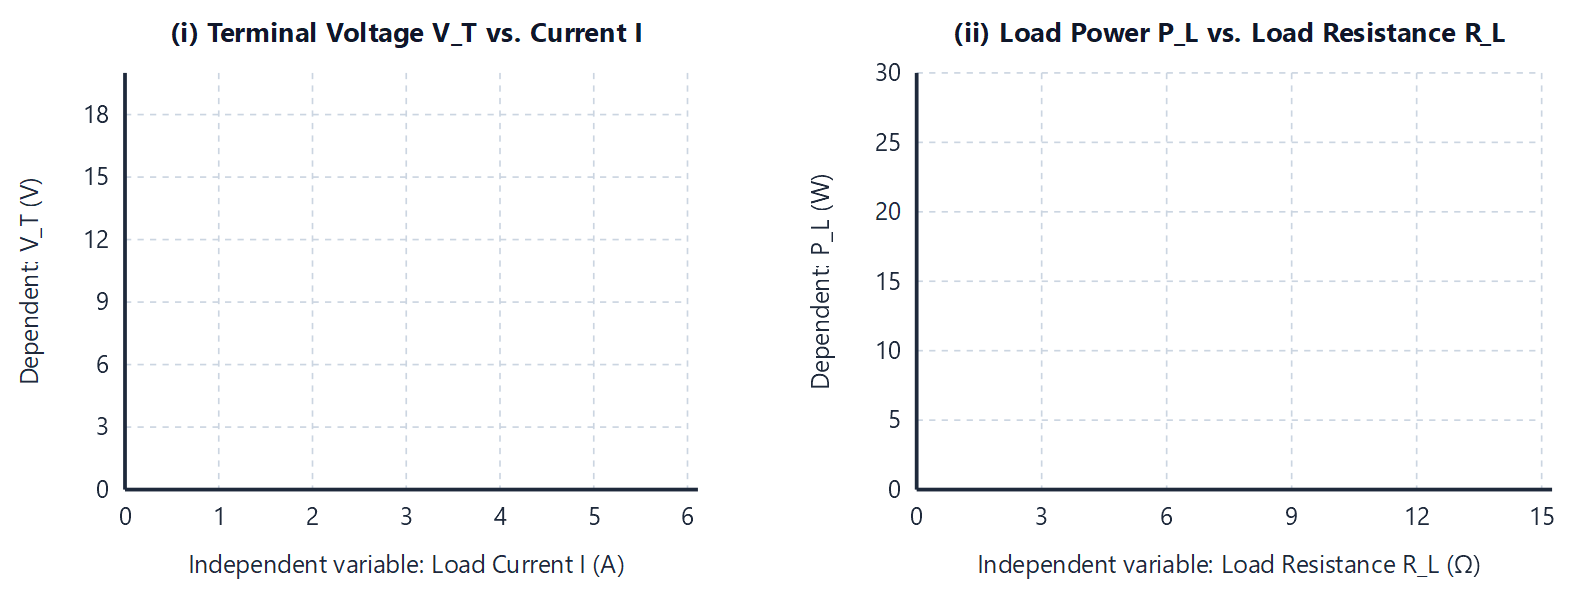
\includegraphics[width=0.96\linewidth]{block_s1_assets/s1-q4-grid-blank.png}\end{center}
\newpage
\section*{Block S2 Exercises: Wheatstone Bridge Analysis via KVL/KCL}

  \textbf{Schedule Window:} Sunday, Oct 18, 4:00--4:55 PM (55 min) ~|~
  \textbf{Total Points:} 34 pts ~|~
  \textbf{Mix:} 1 Calculus/Algebra Derivation, 1 Spec v2 Bridge FR, 1 Graph + Cloze Problem



  \textbf{Core Mastery Goals:} (1) Proving the Wheatstone bridge null-balance ratio $R_1/R_2 = R_3/R_4$ from KCL and KVL; (2) Solving an \emph{unbalanced} bridge where series/parallel formulas fail by writing KCL at the left and right bridge nodes $(V_L, V_R)$ and KVL around meshes containing the central bridge resistor $R_G$; (3) Graphing signed bridge current $I_{LR}(R_4)$ across the balance zero-crossing.


\subsection*{01 $\cdot$ Wheatstone Bridge Null-Balance Condition \& Sensitivity Proof \hfill [Ch. 26 $\cdot$ 10 Points $\cdot$ DERIVE]}

Consider a general DC Wheatstone bridge powered by an ideal source $V_T$ between top node $T$ and grounded bottom node $B$ ($V_B = 0\text{ V}$). Upper-left resistor $R_1$ connects $T \to L$, lower-left resistor $R_2$ connects $L \to B$, upper-right resistor $R_3$ connects $T \to R$, lower-right variable resistor $R_4$ connects $R \to B$, and galvanometer resistance $R_G$ connects $L \to R$ with reference current arrow $I_{LR}$ pointing from $L$ to $R$.

\begin{enumerate}
  \item \textbf{Null-Balance Proof from KCL \& KVL [4 points]:}
    \begin{enumerate}
      \item Suppose the bridge is adjusted so that the galvanometer reads zero current ($I_{LR} = 0$). Using Ohm's law across $R_G$, state the relationship between node potentials $V_L$ and $V_R$, and use KCL at nodes $L$ and $R$ to relate the upper-leg and lower-leg currents ($I_1$ vs. $I_2$, and $I_3$ vs. $I_4$).
      \item Write KVL around the upper loop ($T \to L \to R \to T$) and lower loop ($L \to B \to R \to L$), or apply voltage division on each leg, to prove that $I_{LR} = 0$ if and only if:
      $$\frac{R_1}{R_2} = \frac{R_3}{R_4} \quad \Longleftrightarrow \quad R_1 R_4 = R_2 R_3.$$
      \item Explain briefly why changing the source voltage $V_T$ or the galvanometer resistance $R_G$ does \emph{not} shift the balance resistance $R_{4,\text{bal}}$.
    \end{enumerate}
  
  \item \textbf{Exact Unbalanced Bridge Current \& Calculus Sensitivity Derivative [6 points]:}
    \begin{enumerate}
      \item Fix $V_T = 15.0\text{ V}$, $R_1 = 150\ \Omega$, $R_2 = 300\ \Omega$, $R_3 = 150\ \Omega$, and $R_G = 100\ \Omega$, leaving $R_4 \ge 0$ as a continuous variable. Write KCL at nodes $L$ and $R$ and eliminate $V_L, V_R$ (or find the Th\'evenin equivalent of each bridge leg) to prove that the signed bridge current from $L$ to $R$ is:
      $$I_{LR}(R_4) = \frac{300 - R_4}{6000 + 70 R_4}\text{ A} = \frac{300 - R_4}{6.00 + 0.0700 R_4}\text{ mA}.$$ \textbf{[4 pts]}
      \item Differentiate $I_{LR}(R_4)$ with respect to $R_4$ to evaluate the bridge sensitivity $\left.\dfrac{dI_{LR}}{dR_4}\right|_{R_4 = R_{4,\text{bal}}}$ (in $\mu\text{A}/\Omega$) at the null-balance point. \textbf{[2 pts]}
    \end{enumerate}
  
\end{enumerate}
\vspace{1.2in}


\newpage



\subsection*{02 $\cdot$ Unbalanced Wheatstone Bridge Nodal \& Mesh Analysis \hfill [Ch. 26 $\cdot$ 14 Points $\cdot$ FR + SPEC V2]}

In the Spec v2 Wheatstone bridge below, an ideal DC source $V_T = 15.0\text{ V}$ supplies top node $T$ relative to grounded bottom node $B$ ($V_B = 0\text{ V}$). The four bridge arms are $R_1 = 150\ \Omega$ ($T \to L$), $R_2 = 300\ \Omega$ ($L \to B$), $R_3 = 150\ \Omega$ ($T \to R$), and $R_4 = 150\ \Omega$ ($R \to B$), with central bridge resistor $R_G = 100\ \Omega$ connected between nodes $L$ and $R$.

\begin{center}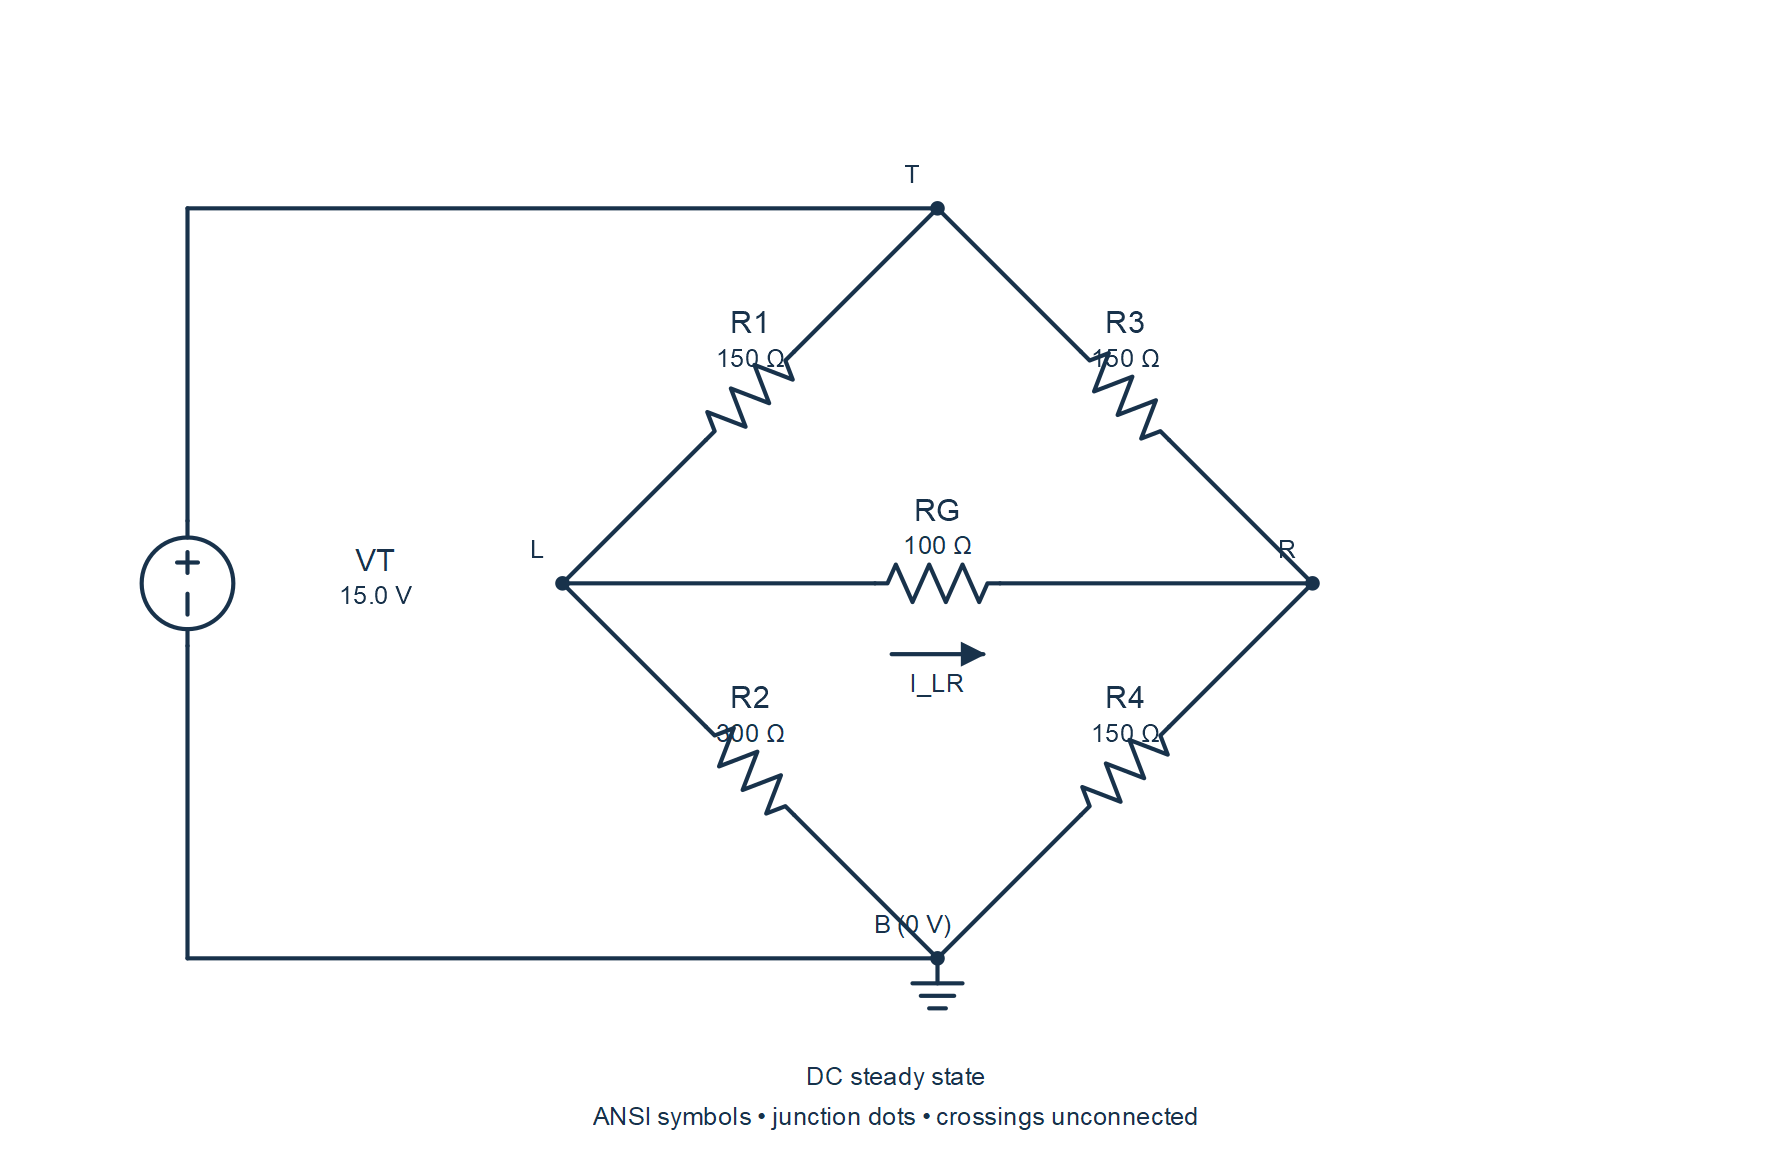
\includegraphics[width=0.82\linewidth]{day1_assets/s2-q2-unbalanced-bridge.png}\end{center}

\begin{enumerate}
  \item \textbf{Why Elementary Series/Parallel Reduction Fails [2 points]:} Explain in one or two sentences why neither $(R_1, R_2)$ nor $(R_1, R_3)$ are in simple series or simple parallel when $R_G = 100\ \Omega$ is present.
  \item \textbf{KCL Nodal System \& KVL Bridge Mesh [4 points]:}
    \begin{enumerate}
      \item Write the KCL equation at node $L$ in terms of the unknown node potentials $V_L$ and $V_R$, and clear fractions to obtain a linear equation of the form $a V_L + b V_R = c$.
      \item Write the KCL equation at node $R$ in terms of $V_L$ and $V_R$, and clear fractions to obtain a second linear equation.
      \item Write the KVL loop equation around the upper triangular mesh ($T \to L \to R \to T$) in terms of branch currents $I_1, I_{LR}, I_3$.
    \end{enumerate}
  
  \item \textbf{Solving for Node Voltages \& Signed Bridge Current [5 points]:} Solve your $2\times 2$ linear system for the exact fractions and three-significant-figure decimal values of $V_L$ and $V_R$ (in $\text{V}$). Calculate the signed bridge current $I_{LR} = \frac{V_L - V_R}{R_G}$ (in $\text{mA}$) and state whether current flows from $L \to R$ or from $R \to L$.
  \item \textbf{All Leg Currents \& Total Equivalent Resistance $R_{\text{eq}}$ [3 points]:} Compute the four leg currents $I_1, I_2, I_3, I_4$ (in $\text{mA}$), find the total source current $I_{\text{src}} = I_1 + I_3 = I_2 + I_4$ leaving node $T$, and determine the total equivalent resistance $R_{\text{eq}} = \frac{V_T}{I_{\text{src}}}$ of the entire 5-resistor bridge network across the $15.0\text{ V}$ source.
\end{enumerate}
\vspace{1.2in}


\newpage



\subsection*{03 $\cdot$ Bridge Current Curve $I_{LR}(R_4)$ \& Conceptual Cloze \hfill [Ch. 26 $\cdot$ 10 Points $\cdot$ DRAW + CLOZE]}

\subsubsection*{Part A: Draw the Effect --- Signed Bridge Current vs. Lower-Right Resistance [6 points --- DRAW]}
Consider the bridge from Exercise 02 ($V_T = 15.0\text{ V}, R_1 = 150\ \Omega, R_2 = 300\ \Omega, R_3 = 150\ \Omega, R_G = 100\ \Omega$) as the lower-right resistor $R_4$ is varied continuously from $0\ \Omega$ to $600\ \Omega$.
\begin{enumerate}
  \item Evaluate $I_{LR}(R_4)$ (in $\text{mA}$) at four landmark resistances: (1) short-circuit $R_4 = 0\ \Omega$, (2) the Exercise 02 operating point $R_4 = 150\ \Omega$, (3) the null-balance resistance $R_{4,\text{bal}}$, and (4) the open-circuit limit $R_4 \to \infty$. \textbf{[2 pts]}
  \item On the coordinate grid below, plot the signed bridge current $I_{LR}$ (\textbf{dependent variable}, vertical axis, in $\text{mA}$) vs. lower-right resistance $R_4$ (\textbf{independent variable}, horizontal axis, in $\Omega$) for $0 \le R_4 \le 600\ \Omega$. Explicitly mark and label the $y$-intercept at $R_4 = 0$, the Exercise 02 operating point at $R_4 = 150\ \Omega$, the zero-crossing balance point at $R_{4,\text{bal}}$, and the dashed horizontal asymptote as $R_4 \to \infty$. \textbf{[4 pts]}
\end{enumerate}

\begin{center}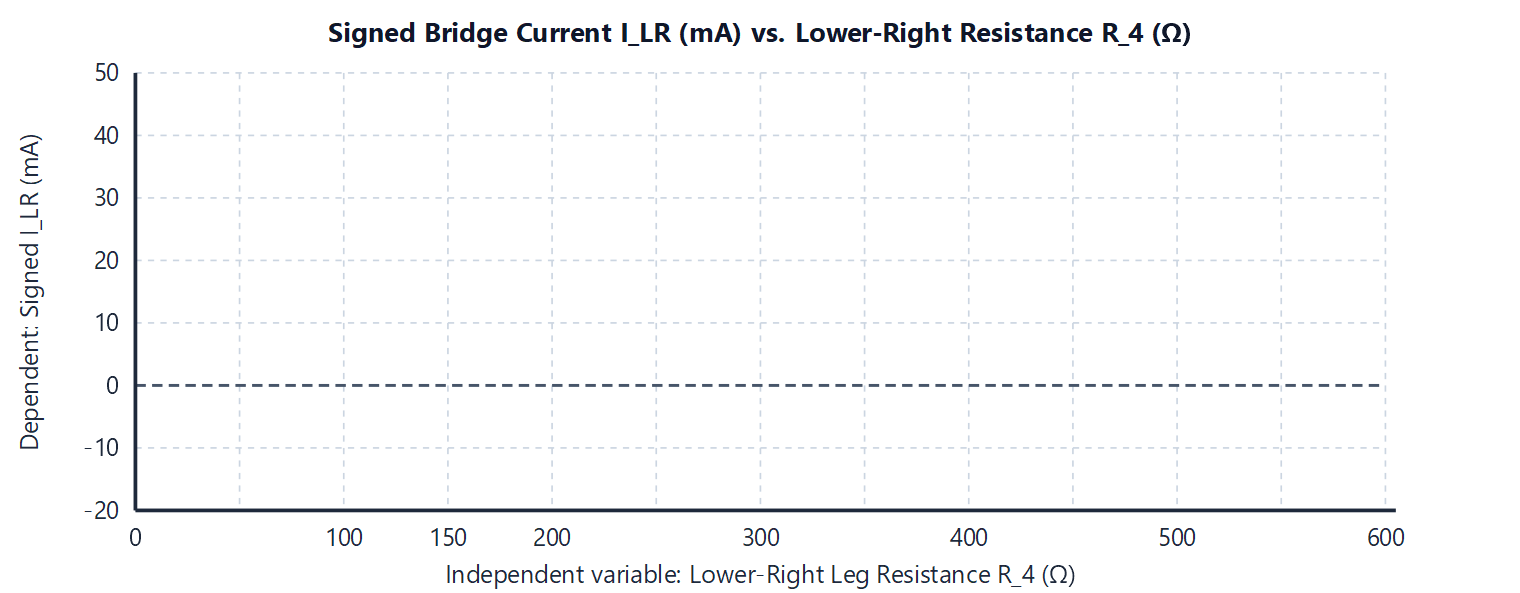
\includegraphics[width=0.82\linewidth]{day1_assets/s2-q3-grid-blank.png}\end{center}

\subsubsection*{Part B: Wheatstone Bridge Conceptual Cloze [4 points --- 0.5 point each]}

  \textbf{WORD BANK:} ~
  \texttt{equal to} $\cdot$
  \texttt{zero} $\cdot$
  \texttt{$300\ \Omega$} $\cdot$
  \texttt{$75.0\ \Omega$} $\cdot$
  \texttt{from $L$ to $R$} $\cdot$
  \texttt{from $R$ to $L$} $\cdot$
  \texttt{unchanged} $\cdot$
  \texttt{doubled} $\cdot$
  \texttt{both an open and a short circuit} $\cdot$
  \texttt{Kirchhoff's junction rule}


\begin{enumerate}
  \item A Wheatstone bridge is balanced when the central galvanometer current $I_G$ is \underline{\hspace{1.8in}}, which requires the node potentials to satisfy $V_L$ \underline{\hspace{1.8in}} $V_R$.
  \item For $R_1 = 150\ \Omega$, $R_2 = 300\ \Omega$, and $R_3 = 150\ \Omega$, the unique lower-right resistance that balances the bridge is $R_{4,\text{bal}} =$ \underline{\hspace{1.8in}}.
  \item When $R_4 < R_{4,\text{bal}}$ (for example, $R_4 = 150\ \Omega$), node $R$ is pulled closer to ground than node $L$ ($V_R < V_L$), so current in $R_G$ flows \underline{\hspace{1.8in}}.
  \item When $R_4 > R_{4,\text{bal}}$ (for example, $R_4 = 500\ \Omega$), $V_R > V_L$ and current in $R_G$ reverses to flow \underline{\hspace{1.8in}}.
  \item If the DC source voltage $V_T$ is doubled from $15.0\text{ V}$ to $30.0\text{ V}$ while the bridge is balanced, the balance resistance $R_{4,\text{bal}}$ remains \underline{\hspace{1.8in}}.
  \item At exact null balance ($I_{LR} = 0$ and $V_L = V_R$), the equivalent resistance $R_{\text{eq}}$ across the source can be found by treating $R_G$ as \underline{\hspace{1.8in}}.
  \item Setting up the nodal equations $\frac{V_L - V_T}{R_1} + \frac{V_L}{R_2} + \frac{V_L - V_R}{R_G} = 0$ is a direct application of \underline{\hspace{1.8in}}.
\end{enumerate}
\newpage
\section*{Block S3 Exercises: RC Charging \& Discharging Transients}

  \textbf{Schedule Window:} Sunday, Oct 18, 5:05--6:05 PM (60 min) ~|~
  \textbf{Total Points:} 40 pts ~|~
  \textbf{Mix:} 2 Calculus Derivations, 1 Two-Stage Switch FR, 1 Aligned Two-Panel Graph



  \textbf{Core Mastery Goals:} (1) Deriving $q(t), v_C(t), i(t)$ by separating variables on the first-order KVL differential equation; (2) Proving by definite integration why a charging resistor dissipates $\frac{1}{2}C\mathcal{E}^2$ regardless of $R$; (3) Applying capacitor voltage continuity $v_C(t_1^+) = v_C(t_1^-)$ and current jump discontinuity across switching events.


\subsection*{01 $\cdot$ First-Order RC Differential Equation \& Separation of Variables \hfill [Ch. 26 $\cdot$ 10 Points $\cdot$ DERIVE]}

An ideal battery of EMF $\mathcal{E} = V_0$ is connected in series with a resistor $R$ and an initially uncharged capacitor $C$ ($q(0) = 0$) as shown in the Spec v2 circuit below, where the switch closes at $t = 0$.

\begin{center}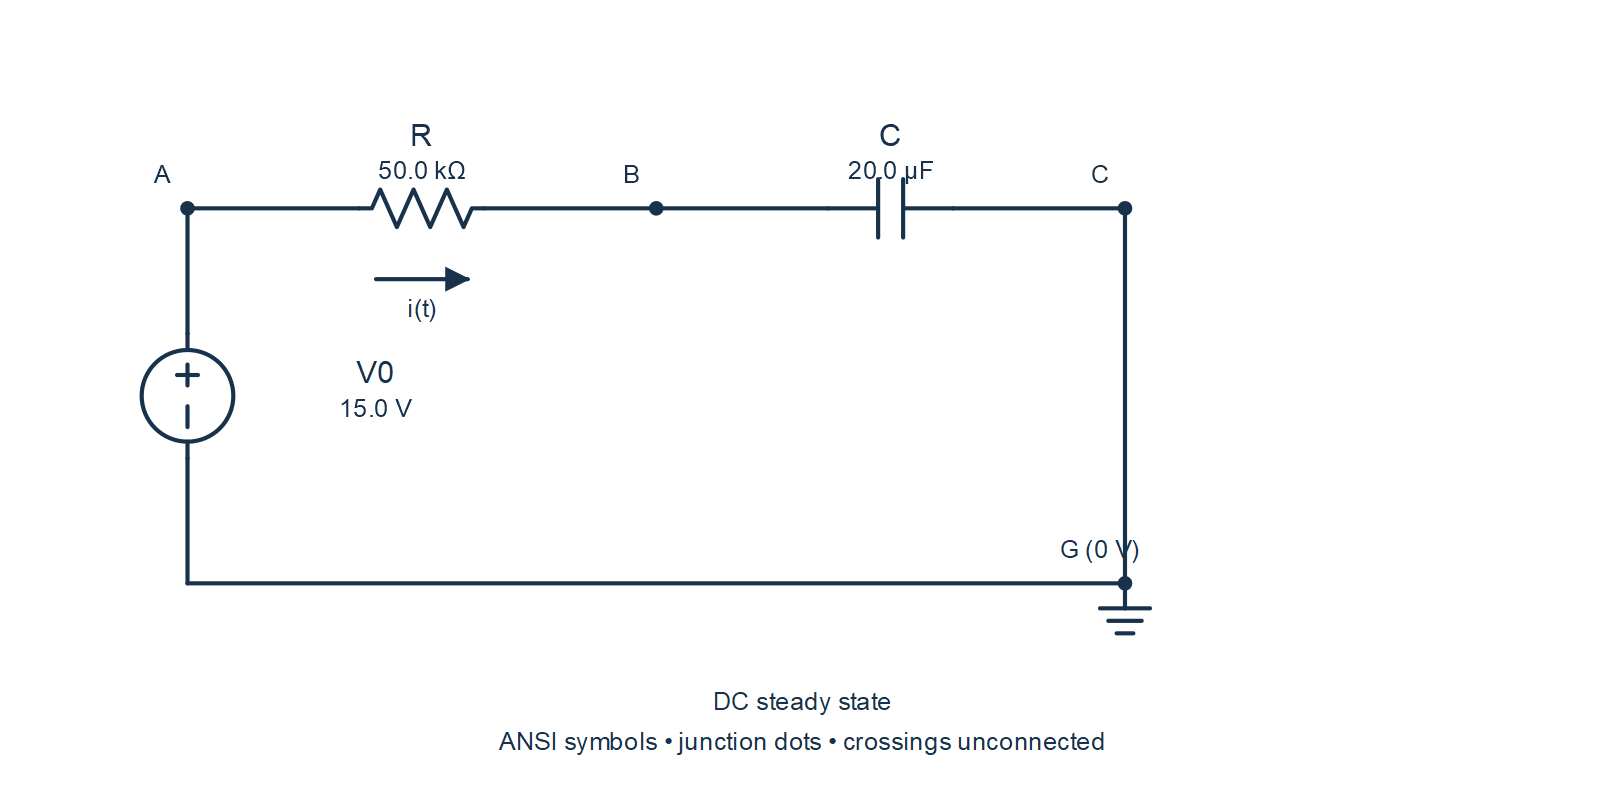
\includegraphics[width=0.82\linewidth]{day1_assets/s3-q1-rc-circuit.png}\end{center}

\begin{enumerate}
  \item \textbf{Charging Differential Equation \& Separation of Variables [6 points]:}
    \begin{enumerate}
      \item Apply Kirchhoff's loop rule around the series circuit for $t \ge 0$ and substitute $i(t) = \dfrac{dq}{dt}$ to write the first-order linear differential equation for $q(t)$. \textbf{[2 pts]}
      \item Separate variables so that all $q$-dependent terms are on the left and all $t$-dependent terms are on the right, and integrate explicitly from $q(0) = 0$ at $t' = 0$ to $q(t)$ at $t' = t$:
      $$\int_{0}^{q(t)} \frac{dq'}{C\mathcal{E} - q'} = \int_{0}^{t} \frac{dt'}{RC}.$$
      Solve for $q(t)$, $v_C(t) = \frac{q(t)}{C}$, and $i(t) = \frac{dq}{dt}$, identifying the capacitive time constant $\tau = RC$. \textbf{[4 pts]}
    \end{enumerate}
  
  \item \textbf{Discharging from Initial Charge $Q_0$ [4 points]:} Suppose the battery is removed and a capacitor carrying initial charge $Q_0 = C V_{\text{init}}$ at $t = 0$ is discharged through resistor $R$. Write the KVL differential equation $\frac{q}{C} + R\frac{dq}{dt} = 0$, separate variables, and integrate from $Q_0$ to $q(t)$ to derive $q(t) = Q_0 e^{-t/RC}$ and $v_C(t) = V_{\text{init}} e^{-t/RC}$.
\end{enumerate}
\vspace{1.2in}


\newpage



\subsection*{02 $\cdot$ Calculus Proof of Energy Conservation \& Half-Energy Dissipation \hfill [Ch. 24, 26 $\cdot$ 10 Points $\cdot$ DERIVE]}

When an initially uncharged capacitor $C$ is charged to final voltage $\mathcal{E}$ through a series resistor $R$ by a constant-EMF battery $\mathcal{E}$, the charging current is $i(t) = \dfrac{\mathcal{E}}{R} e^{-t/(RC)}$ for $0 \le t < \infty$.

\begin{enumerate}
  \item \textbf{Total Charge \& Work Done by the Battery [3 points]:}
    \begin{enumerate}
      \item Integrate the current from $t = 0$ to $t \to \infty$ to verify that the total charge delivered by the battery is $Q_{\text{final}} = \int_0^\infty i(t)\,dt = C\mathcal{E}$.
      \item Using $dW_{\text{batt}} = \mathcal{E}\,dq = \mathcal{E} i(t)\,dt$, show that the total electrical work done by the battery over the entire charging process is:
      $$W_{\text{batt}} = \int_{0}^{\infty} \mathcal{E} i(t)\,dt = C\mathcal{E}^2.$$
    \end{enumerate}
  
  \item \textbf{Joule Heating Integral in the Resistor [5 points]:} The instantaneous rate of thermal energy dissipation in the resistor is $P_R(t) = [i(t)]^2 R$. Set up and evaluate the improper integral:
  $$E_{\text{dissipated}} = \int_{0}^{\infty} [i(t)]^2 R\,dt = \int_{0}^{\infty} \left(\frac{\mathcal{E}}{R} e^{-t/(RC)}\right)^2 R\,dt$$
  to prove that:
  $$E_{\text{dissipated}} = \frac{1}{2} C\mathcal{E}^2.$$
  \item \textbf{Energy Accounting \& Physical Independence from $R$ [2 points]:} Compare $E_{\text{dissipated}}$ with the final electrostatic energy $U_C = \int_0^{C\mathcal{E}} \frac{q}{C}\,dq = \frac{1}{2}C\mathcal{E}^2$ stored in the capacitor, verify $W_{\text{batt}} = U_C + E_{\text{dissipated}}$, and explain mathematically why the resistance $R$ cancels out of $E_{\text{dissipated}}$ (what happens to peak power vs. duration $\tau = RC$ if $R$ is halved?).
\end{enumerate}
\vspace{1.2in}


\newpage



\subsection*{03 $\cdot$ Two-Position Switch RC Transient \& Continuity vs. Jump Analysis \hfill [Ch. 26 $\cdot$ 10 Points $\cdot$ FR + SWITCH]}

In the two-position switch circuit below, $V_0 = 15.0\text{ V}$, $R = 50.0\text{ k}\Omega$, and $C = 20.0\ \mu\text{F}$. The capacitor is initially uncharged ($v_C(0^-) = 0\text{ V}$). At $t = 0$, switch $S$ is thrown to \textbf{Position 1} (connecting the series $RC$ branch to $V_0 = 15.0\text{ V}$) and remains there for $0 \le t < 2.00\text{ s}$. At instant $t_1 = 2.00\text{ s}$, switch $S$ is thrown instantaneously to \textbf{Position 2} (connecting the left end of $R$ directly to ground, $0\text{ V}$, for $t \ge 2.00\text{ s}$). The reference current $i(t) = C\frac{dv_C}{dt}$ is defined flowing rightward into the top plate (Node $B$).

\begin{center}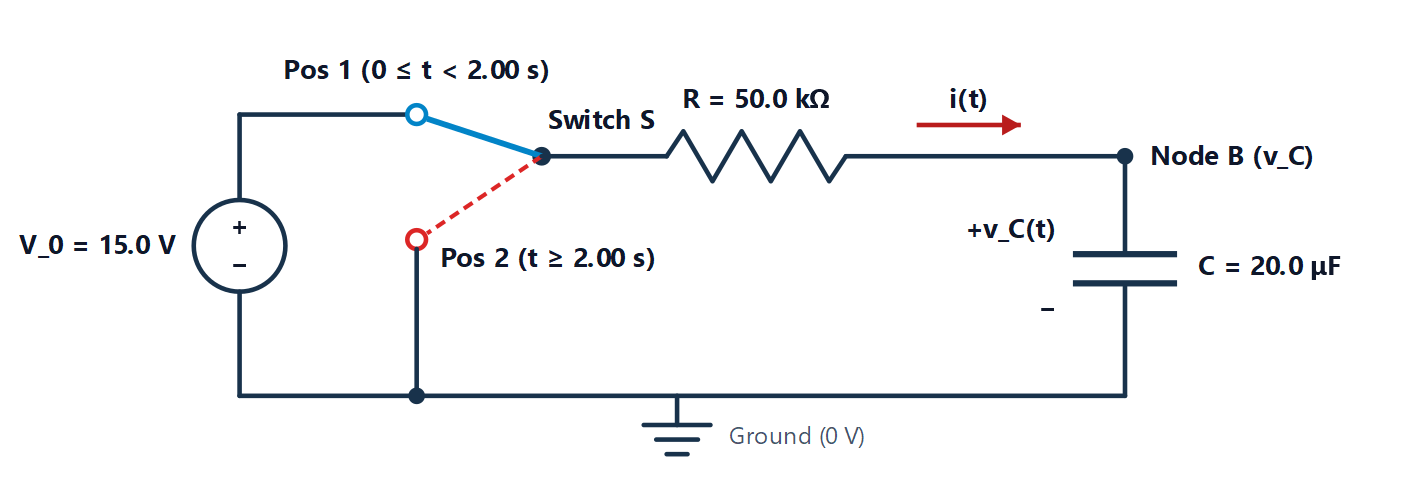
\includegraphics[width=0.82\linewidth]{day1_assets/s3-q3-rc-switch.png}\end{center}

\begin{enumerate}
  \item \textbf{Time Constant \& Initial Charging ($t = 0^+$) [2 points]:} Compute the capacitive time constant $\tau = RC$ (in $\text{s}$), the initial capacitor voltage $v_C(0^+)$, and the initial charging current $i(0^+)$ (in $\mu\text{A}$).
  \item \textbf{State Just Before Switching ($t_1^- = 2.00\text{ s}^-$) [3 points]:} Write the analytical expressions for $v_C(t)$ and $i(t)$ on $0 \le t < 2.00\text{ s}$, and calculate the numerical values of $v_C(2.00\text{ s}^-)$ (in $\text{V}$) and $i(2.00\text{ s}^-)$ (in $\mu\text{A}$).
  \item \textbf{Switching Instant Continuity \& Jump ($t_1^+ = 2.00\text{ s}^+$) [3 points]:}
    \begin{enumerate}
      \item State the value of $v_C(2.00\text{ s}^+)$ immediately after the switch moves to Position 2, and explain physically why $v_C(t)$ cannot jump instantaneously when $R > 0$.
      \item Calculate the signed current $i(2.00\text{ s}^+)$ (in $\mu\text{A}$) immediately after switching to Position 2, and compute the instantaneous jump $\Delta i = i(2.00\text{ s}^+) - i(2.00\text{ s}^-)$.
    \end{enumerate}
  
  \item \textbf{Discharging Regime ($t \ge 2.00\text{ s}$) [2 points]:} Write $v_C(t)$ and $i(t)$ as functions of $(t - 2.00\text{ s})$ for $t \ge 2.00\text{ s}$, and evaluate $v_C(3.50\text{ s})$ (in $\text{V}$) and $i(3.50\text{ s})$ (in $\mu\text{A}$).
\end{enumerate}
\vspace{1.2in}


\newpage



\subsection*{04 $\cdot$ Aligned $v_C(t)$ and $i(t)$ Transient Graphs \& Continuity Cloze \hfill [Ch. 26 $\cdot$ 10 Points $\cdot$ DRAW + CLOZE]}

\subsubsection*{Part A: Draw the Effect --- Aligned Two-Panel Transient Plots [6 points --- DRAW]}
For the two-stage switching circuit of Exercise 03 ($V_0 = 15.0\text{ V}, R = 50.0\text{ k}\Omega, C = 20.0\ \mu\text{F}$, switch thrown from Position 1 to Position 2 at $t_1 = 2.00\text{ s}$):
\begin{enumerate}
  \item \textbf{Graph (i) [3 points]:} On the left grid below, plot the capacitor voltage $v_C(t)$ (\textbf{dependent variable}, vertical axis, in $\text{V}$) vs. time $t$ (\textbf{independent variable}, horizontal axis, in $\text{s}$) from $t = 0$ to $t = 5.00\text{ s}$. Label the coordinates of the cusp peak at $t_1 = 2.00\text{ s}$ and the value at $t = 3.50\text{ s}$ using your results from Exercise 03.
  \item \textbf{Graph (ii) [3 points]:} On the right grid below, plot the signed current $i(t) = C\frac{dv_C}{dt}$ (\textbf{dependent variable}, vertical axis, in $\mu\text{A}$) vs. time $t$ (\textbf{independent variable}, horizontal axis, in $\text{s}$) from $t = 0$ to $t = 5.00\text{ s}$. Mark and label the initial current $i(0^+)$, the pre-switch current $i(2.00\text{ s}^-)$, the post-switch current $i(2.00\text{ s}^+)$, and the value $i(3.50\text{ s})$ calculated in Exercise 03.
\end{enumerate}

\begin{center}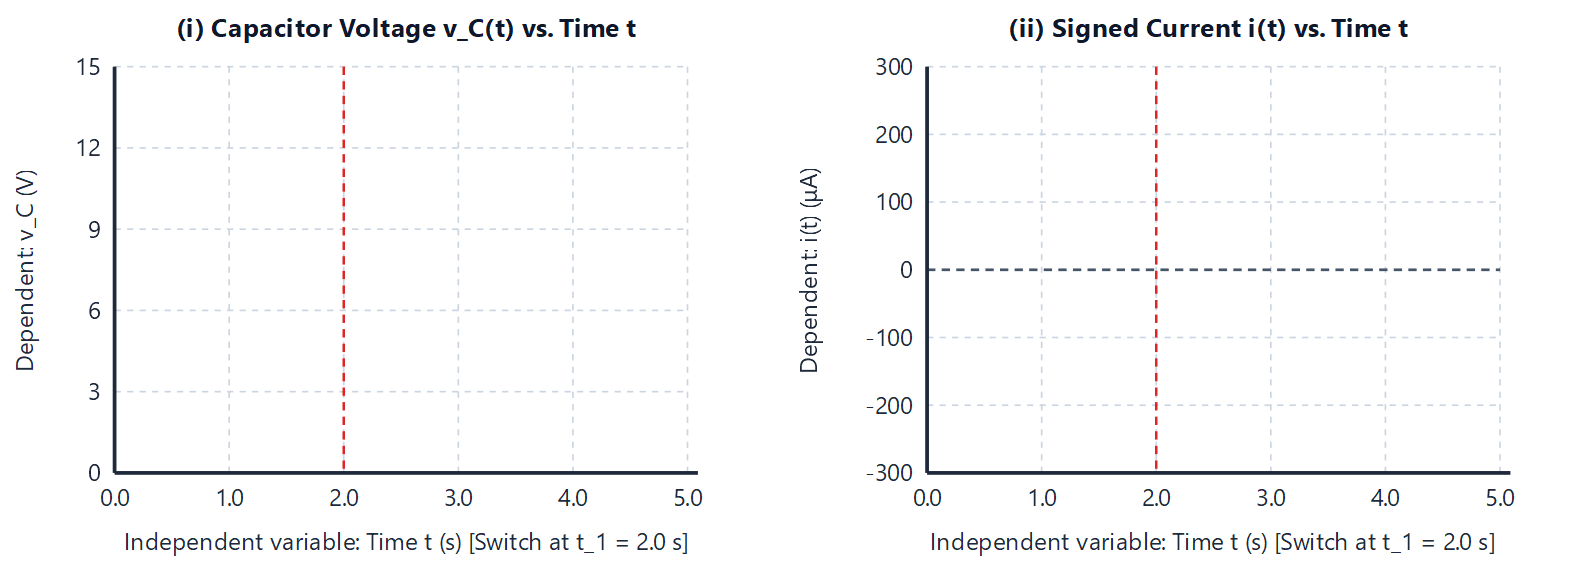
\includegraphics[width=0.82\linewidth]{day1_assets/s3-q4-grid-blank.png}\end{center}

\subsubsection*{Part B: RC Transient \& Continuity Rules Cloze [4 points --- 0.5 point each]}

  \textbf{WORD BANK:} ~
  \texttt{short circuit (wire)} $\cdot$
  \texttt{open circuit} $\cdot$
  \texttt{continuous} $\cdot$
  \texttt{discontinuous} $\cdot$
  \texttt{$63.2\\%$} $\cdot$
  \texttt{$36.8\\%$} $\cdot$
  \texttt{$86.5\\%$} $\cdot$
  \texttt{$\frac{1}{2}C\mathcal{E}^2$} $\cdot$
  \texttt{$C\mathcal{E}^2$} $\cdot$
  \texttt{seconds ($\text{s}$)}


\begin{enumerate}
  \item In SI units, the product $\tau = RC$ has dimensions of $(\text{V/A})\cdot(\text{C/V}) = \text{C/(C/s)}$, which reduces to \underline{\hspace{1.8in}}.
  \item At $t = 0^+$ immediately after a DC source is connected to an uncharged capacitor ($q(0^+)=0 \implies v_C(0^+)=0$), the capacitor momentarily behaves as a \underline{\hspace{1.8in}}.
  \item As $t \to \infty$ in DC steady state, a fully charged capacitor carries zero current ($i(\infty)=0$) and behaves as an \underline{\hspace{1.8in}}.
  \item After one time constant ($t = \tau = RC$) of charging from zero, $v_C(\tau)$ reaches $1 - e^{-1} \approx$ \underline{\hspace{1.8in}} of its final asymptotic voltage $\mathcal{E}$, while the charging current $i(\tau)$ decays to $e^{-1} \approx$ \underline{\hspace{1.8in}} of $i(0^+)$.
  \item Across any finite-current switching instant $t = t_1$, the capacitor voltage $v_C(t)$ must be \underline{\hspace{1.8in}}, whereas the resistor current $i(t)$ is generally \underline{\hspace{1.8in}}.
  \item During complete charging of an uncharged capacitor $C$ from an ideal battery $\mathcal{E}$, the total thermal energy dissipated in the series resistor $R$ is always \underline{\hspace{1.8in}}.
\end{enumerate}
\newpage
\section*{Block S4 Exercises: DC-Driven Series RLC Circuit Analysis}

  \textbf{Schedule Window:} Sunday, Oct 18, 6:50--7:50 PM (60 min) ~|~
  \textbf{Total Points:} 36 pts ~|~
  \textbf{Mix:} 1 Second-Order ODE Derivation, 1 Spec v2 RLC Step-Response FR, 1 Damping Graph + Cloze



  \textbf{Core Mastery Goals:} (1) Deriving the second-order ODE $LC\frac{d^2 v_C}{dt^2} + RC\frac{dv_C}{dt} + v_C = V_s$, characteristic roots, critical damping resistance $R_{\text{crit}} = 2\sqrt{L/C}$, and ringing frequency $\omega' = \sqrt{\frac{1}{LC} - \frac{R^2}{4L^2}}$; (2) Enforcing dual continuity $v_C(0^+)=v_C(0^-)$ and $i_L(0^+)=i_L(0^-)$ alongside DC steady-state limits ($t \to \infty$: $C =$ open, $L =$ short); (3) Sketching underdamped, critically damped, and overdamped step responses.


\subsection*{01 $\cdot$ Second-Order Series RLC ODE, Characteristic Roots \& Critical Damping Proof \hfill [Ch. 30 $\cdot$ 12 Points $\cdot$ DERIVE]}

A constant DC voltage source $V_s = \mathcal{E}$ is switched at $t = 0$ into a series circuit containing resistance $R$, inductance $L$, and capacitance $C$.

\begin{enumerate}
  \item \textbf{Second-Order Differential Equation in $v_C(t)$ [4 points]:}
    \begin{enumerate}
      \item Write Kirchhoff's loop rule for $t \ge 0$ in terms of the loop current $i(t)$, $\dfrac{di}{dt}$, and the capacitor voltage $v_C(t)$.
      \item Using $q(t) = C v_C(t)$, express $i(t) = \dfrac{dq}{dt}$ and $\dfrac{di}{dt} = \dfrac{d^2 q}{dt^2}$ in terms of derivatives of $v_C(t)$, and substitute them into KVL to prove that $v_C(t)$ satisfies the second-order linear ODE:
      $$LC\frac{d^2 v_C}{dt^2} + RC\frac{dv_C}{dt} + v_C = \mathcal{E} \quad \Longleftrightarrow \quad \frac{d^2 v_C}{dt^2} + \frac{R}{L}\frac{dv_C}{dt} + \frac{1}{LC}v_C = \frac{\mathcal{E}}{LC}.$$
    \end{enumerate}
  
  \item \textbf{Characteristic Equation, Damping Regimes \& $R_{\text{crit}}$ [5 points]:}
    \begin{enumerate}
      \item Substitute the trial homogeneous solution $v_{C,h}(t) = A e^{st}$ into the homogeneous ODE $\frac{d^2 v_{C,h}}{dt^2} + \frac{R}{L}\frac{dv_{C,h}}{dt} + \frac{1}{LC}v_{C,h} = 0$ to obtain the quadratic characteristic equation in $s$, and solve for the roots $s_{1,2}$ in terms of the attenuation constant $\alpha = \dfrac{R}{2L}$ and the undamped natural angular frequency $\omega_0 = \dfrac{1}{\sqrt{LC}}$.
      \item Set the discriminant $\alpha^2 - \omega_0^2 = 0$ to prove that the boundary between oscillatory (underdamped) and non-oscillatory (overdamped) response occurs at the \textbf{critical damping resistance}:
      $$R_{\text{crit}} = 2\sqrt{\frac{L}{C}}.$$
    \end{enumerate}
  
  \item \textbf{Underdamped Ringing Frequency $\omega'$ [3 points]:} When $R < R_{\text{crit}}$, show that the characteristic roots are complex conjugates $s_{1,2} = -\alpha \pm j\omega'$ with damped angular frequency:
  $$\omega' = \sqrt{\omega_0^2 - \alpha^2} = \sqrt{\frac{1}{LC} - \frac{R^2}{4L^2}},$$
  and verify that the general underdamped step response satisfying $v_C(0^+)=0$, $\left.\frac{dv_C}{dt}\right|_{0^+}=0$, and $v_C(\infty)=\mathcal{E}$ is $v_C(t) = \mathcal{E}\left[1 - e^{-\alpha t}\left(\cos(\omega' t) + \frac{\alpha}{\omega'}\sin(\omega' t)\right)\right]$.
\end{enumerate}
\vspace{1.2in}


\newpage



\subsection*{02 $\cdot$ DC Step-Response Continuity ($t=0^+$), Steady State ($t\to\infty$) \& Damping \hfill [Ch. 30 $\cdot$ 14 Points $\cdot$ FR + SPEC V2]}

In the Spec v2 series RLC circuit below, an ideal DC source $V_s = 12.0\text{ V}$ is applied at $t = 0$ to a series combination of $R = 40.0\ \Omega$, $L = 0.800\text{ H}$, and $C = 500\ \mu\text{F}$. Prior to $t = 0$, the capacitor is completely uncharged ($v_C(0^-) = 0\text{ V}$) and the inductor carries zero current ($i(0^-) = 0\text{ A}$).

\begin{center}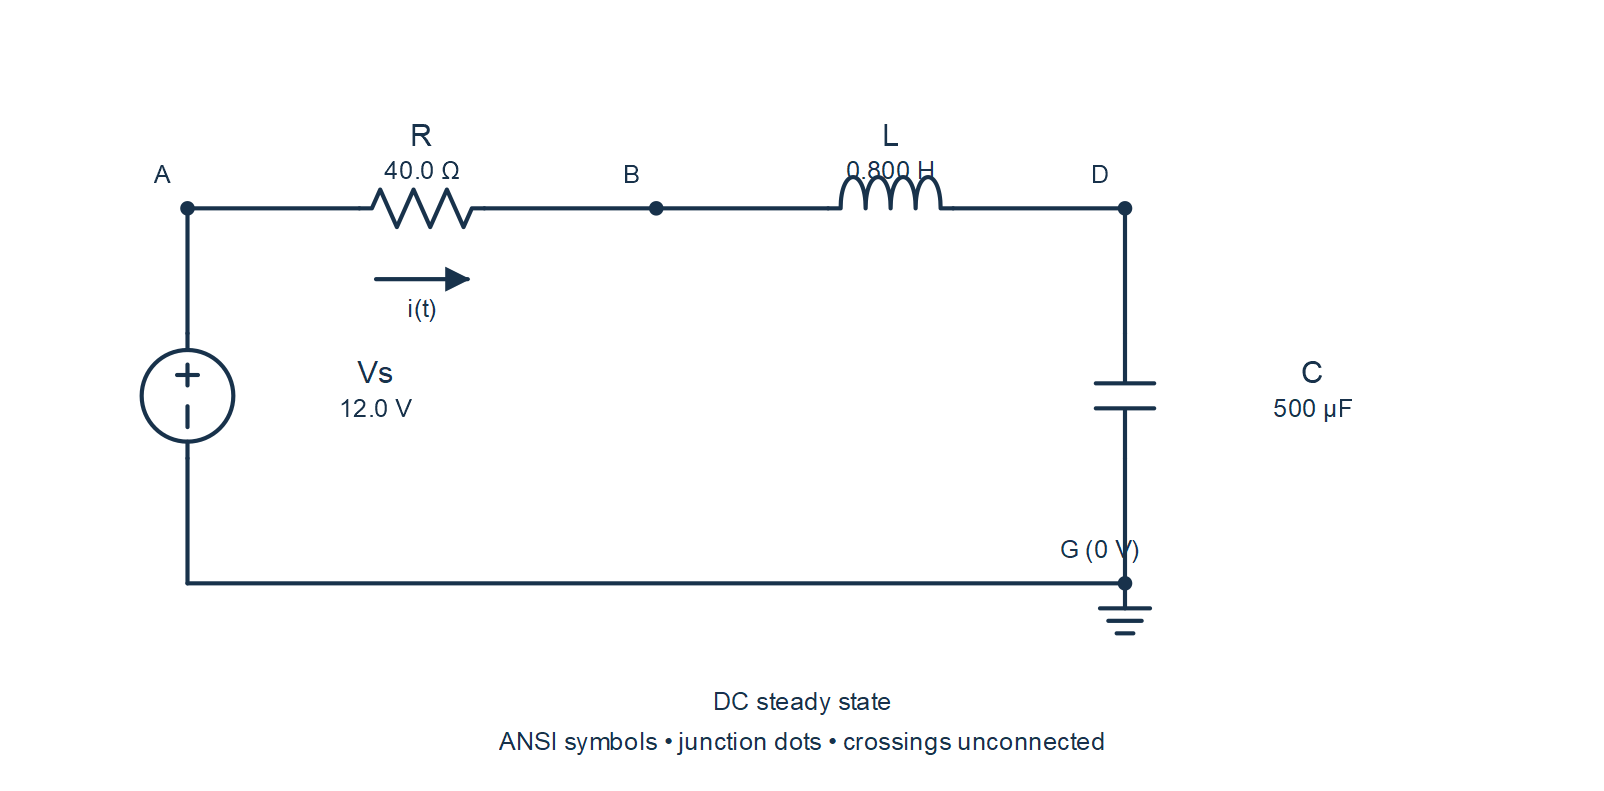
\includegraphics[width=0.82\linewidth]{day1_assets/s4-q2-dc-rlc.png}\end{center}

\begin{enumerate}
  \item \textbf{Initial State Immediately After Switching ($t = 0^+$) [5 points]:}
    \begin{enumerate}
      \item Using the physical continuity rules for an inductor and a capacitor, state $i(0^+)$ (in $\text{A}$) and $v_C(0^+)$ (in $\text{V}$).
      \item Find the initial resistor voltage $v_R(0^+)$ and apply KVL at $t = 0^+$ to determine the initial inductor voltage $v_L(0^+)$ (in $\text{V}$).
      \item Calculate the initial rate of change of current $\left.\dfrac{di}{dt}\right|_{t=0^+}$ (in $\text{A/s}$), the initial rate of change of capacitor voltage $\left.\dfrac{dv_C}{dt}\right|_{t=0^+}$ (in $\text{V/s}$), and the initial second derivative $\left.\dfrac{d^2 v_C}{dt^2}\right|_{t=0^+}$ (in $\text{V/s}^2$).
    \end{enumerate}
  
  \item \textbf{Final DC Steady State ($t \to \infty$) \& Stored Energy [4 points]:}
    \begin{enumerate}
      \item As $t \to \infty$ (after all transients have died out), state the asymptotic circuit model (open circuit vs. short circuit) for $L$ and for $C$, and determine $i(\infty)$, $v_R(\infty)$, $v_L(\infty)$, and $v_C(\infty)$.
      \item Compute the final magnetic energy stored in the inductor $U_L(\infty) = \frac{1}{2}L[i(\infty)]^2$ and the final electric energy stored in the capacitor $U_C(\infty) = \frac{1}{2}C[v_C(\infty)]^2$ (in $\text{mJ}$).
    \end{enumerate}
  
  \item \textbf{Damping Classification \& Peak Overshoot [5 points]:}
    \begin{enumerate}
      \item Calculate the undamped natural frequency $\omega_0 = \frac{1}{\sqrt{LC}}$ (in $\text{rad/s}$), the damping coefficient $\alpha = \frac{R}{2L}$ (in $\text{s}^{-1}$), and the critical damping resistance $R_{\text{crit}} = 2\sqrt{\frac{L}{C}}$ (in $\Omega$).
      \item Classify the circuit at $R = 40.0\ \Omega$ as \emph{underdamped}, \emph{critically damped}, or \emph{overdamped}, compute the damped ringing frequency $\omega' = \sqrt{\omega_0^2 - \alpha^2}$ (in $\text{rad/s}$), and find the time $t_{\text{peak}} = \frac{\pi}{\omega'}$ (in $\text{ms}$) and maximum capacitor voltage $v_{C,\max} = v_C(t_{\text{peak}})$ (in $\text{V}$) at the first overshoot peak.
    \end{enumerate}
  
\end{enumerate}
\vspace{1.2in}


\newpage



\subsection*{03 $\cdot$ Step-Response Damping Curves \& RLC Continuity Cloze \hfill [Ch. 30 $\cdot$ 10 Points $\cdot$ DRAW + CLOZE]}

\subsubsection*{Part A: Draw the Effect --- Underdamped, Critically Damped \& Overdamped Step Responses [6 points --- DRAW]}
For the series RLC circuit of Exercise 02 ($V_s = 12.0\text{ V}, L = 0.800\text{ H}, C = 500\ \mu\text{F}$), sketch on the same coordinate axes below the capacitor voltage $v_C(t)$ (\textbf{dependent variable}, vertical axis, in $\text{V}$) vs. time $t$ (\textbf{independent variable}, horizontal axis, in $\text{ms}$) for $0 \le t \le 150\text{ ms}$ for three different series resistances, identifying the damping regime of each curve:
\begin{enumerate}
  \item \textbf{Curve 1 (Solid): $R_1 = 40.0\ \Omega$} --- state the damping regime, draw the dashed horizontal steady-state asymptote $v_C(\infty)$, and mark the initial slope at $t = 0^+$ along with the coordinates $(t_{\text{peak}}, v_{C,\max})$ of any first peak found in Exercise 02. \textbf{[2.5 pts]}
  \item \textbf{Curve 2 (Dashed): $R_2 = 80.0\ \Omega$} --- state the damping regime and sketch its time response relative to Curve 1 and $v_C(\infty)$. \textbf{[2 pts]}
  \item \textbf{Curve 3 (Dotted): $R_3 = 160\ \Omega$} --- state the damping regime and sketch its time response relative to Curves 1 and 2. \textbf{[1.5 pts]}
\end{enumerate}

\begin{center}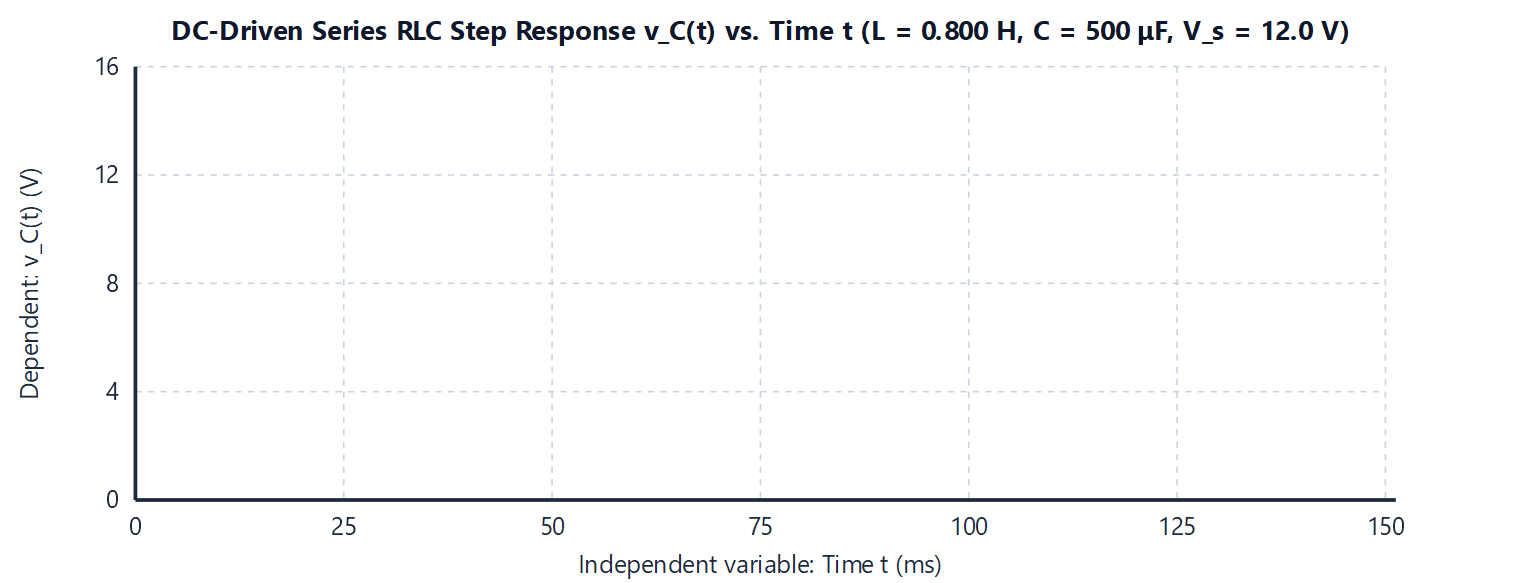
\includegraphics[width=0.82\linewidth]{day1_assets/s4-q3-grid-blank.png}\end{center}

\subsubsection*{Part B: DC-Driven RLC Continuity \& Damping Cloze [4 points --- 0.5 point each]}

  \textbf{WORD BANK:} ~
  \texttt{inductor current $i_L(t)$} $\cdot$
  \texttt{inductor voltage $v_L(t)$} $\cdot$
  \texttt{open circuit} $\cdot$
  \texttt{short circuit} $\cdot$
  \texttt{underdamped} $\cdot$
  \texttt{critically damped} $\cdot$
  \texttt{overdamped} $\cdot$
  \texttt{$2\sqrt{L/C}$} $\cdot$
  \texttt{$1/\sqrt{LC}$} $\cdot$
  \texttt{zero}


\begin{enumerate}
  \item Because magnetic flux linkage $\Phi_B = L i_L$ cannot change instantaneously under a finite voltage ($v_L = L\frac{di_L}{dt}$), the \underline{\hspace{1.8in}} must be continuous across any switching instant, whereas the \underline{\hspace{1.8in}} can jump discontinuously.
  \item At $t = 0^+$ when a DC step voltage is applied to a de-energized inductor ($i_L(0^+)=0$), the inductor momentarily acts like an \underline{\hspace{1.8in}}; as $t \to \infty$ in DC steady state ($\frac{di_L}{dt} = 0$), the ideal inductor acts like a \underline{\hspace{1.8in}}.
  \item Because $i(0^+) = C\left.\frac{dv_C}{dt}\right|_{0^+} = 0$ in a initially de-energized series RLC circuit, the initial slope of the $v_C(t)$ graph at $t = 0^+$ is always \underline{\hspace{1.8in}} for all damping regimes.
  \item The boundary between oscillatory ringing and non-oscillatory decay occurs at $R_{\text{crit}} =$ \underline{\hspace{1.8in}}.
  \item When $0 < R < R_{\text{crit}}$, the circuit is \underline{\hspace{1.8in}} and $v_C(t)$ overshoots and rings around $V_s$; when $R = R_{\text{crit}}$, the circuit is \underline{\hspace{1.8in}} and approaches $V_s$ as rapidly as possible without overshooting.
\end{enumerate}
\newpage
\section*{Block S5 Exercises: Series AC RLC Concepts, Inductance, Reactance \& Capacitance}

  \textbf{Schedule Window:} Sunday, Oct 18, 8:00--9:00 PM (60 min) ~|~
  \textbf{Total Points:} 44 pts ~|~
  \textbf{Mix:} 2 Calculus Derivations, 1 10-Blank Cloze, 1 Spec v2 AC RLC FR, 2 Graphs + Phasors



  \textbf{Core Mastery Goals:} (1) Deriving $X_L = \omega L$ ($+90^\circ$ voltage lead) and $X_C = \frac{1}{\omega C}$ ($-90^\circ$ voltage lag) from $v_L = L\frac{di}{dt}$ and $i_C = C\frac{dv_C}{dt}$; (2) Deriving solenoid inductance $L = \frac{\mu_0 N^2 A}{\ell}$ and magnetic energy density $u_B = \frac{B^2}{2\mu_0}$; (3) Mastering series impedance $Z = \sqrt{R^2 + (X_L - X_C)^2}$, phase angle $\phi$, and series resonance $\omega_0 = \frac{1}{\sqrt{LC}}$.


\subsection*{01 $\cdot$ Calculus Proofs: Inductive/Capacitive Reactance \& Solenoid Energy Density \hfill [Ch. 30--31 $\cdot$ 12 Points $\cdot$ DERIVE]}

\begin{enumerate}
  \item \textbf{Inductive Reactance $X_L = \omega L$ \& Capacitive Reactance $X_C = \frac{1}{\omega C}$ [6 points]:} Suppose a steady sinusoidal AC current $i(t) = I_0 \cos(\omega t)$ with angular frequency $\omega$ (in $\text{rad/s}$) and amplitude $I_0$ flows through a series circuit.
    \begin{enumerate}
      \item Substitute $i(t) = I_0\cos(\omega t)$ into Faraday's inductor relation $v_L(t) = L\dfrac{di}{dt}$, use the trigonometric identity $-\sin(\omega t) = \cos(\omega t + \frac{\pi}{2})$, and prove that the peak inductor voltage is $V_{L,0} = I_0 X_L$ where $X_L = \omega L$, with $v_L(t)$ \textbf{leading} $i(t)$ by $+90^\circ$ ($+\frac{\pi}{2}\text{ rad}$). \textbf{[3 pts]}
      \item Integrate $v_C(t) = \dfrac{1}{C}\int i(t)\,dt$ (with zero DC offset) or differentiate $i(t) = C\dfrac{dv_C}{dt}$, use $\sin(\omega t) = \cos(\omega t - \frac{\pi}{2})$, and prove that the peak capacitor voltage is $V_{C,0} = I_0 X_C$ where $X_C = \dfrac{1}{\omega C}$, with $v_C(t)$ \textbf{lagging} $i(t)$ by $-90^\circ$ ($-\frac{\pi}{2}\text{ rad}$). \textbf{[3 pts]}
    \end{enumerate}
  
  \item \textbf{Solenoid Self-Inductance \& Magnetic Field Energy Density [6 points]:} Consider a long, tightly wound ideal solenoid of length $\ell$, cross-sectional area $A$, and $N$ total turns carrying current $I$, as shown below.
  \begin{center}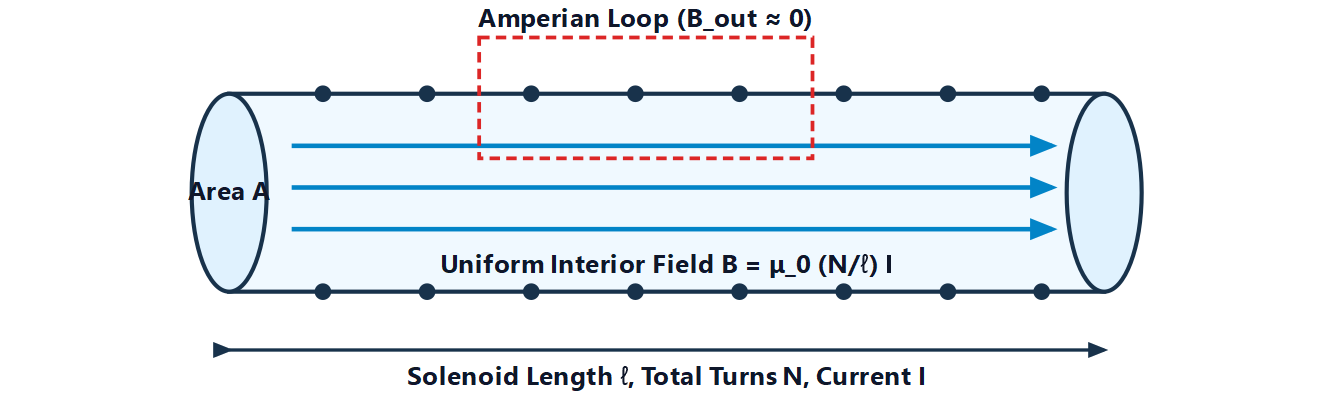
\includegraphics[width=0.82\linewidth]{day1_assets/s5-q1-solenoid.png}\end{center}
    \begin{enumerate}
      \item Apply Amp\`ere's law $\oint \mathbf{B}\cdot d\mathbf{l} = \mu_0 I_{\text{enc}}$ around the dashed rectangular Amperian loop to find the uniform interior magnetic field $B$, compute the total flux linkage $N\Phi_B = N(BA)$, and prove from $N\Phi_B = LI$ that the solenoid's self-inductance is:
      $$L = \frac{\mu_0 N^2 A}{\ell}.$$ \textbf{[3 pts]}
      \item Integrate the instantaneous magnetic power $dU_B = v_L i\,dt = L i\,di$ from $i' = 0$ to $i' = I$ to prove $U_B = \frac{1}{2}LI^2$, and divide by the interior volume $V_{\text{vol}} = A\ell$ to prove that the magnetic energy density stored in any magnetic field $B$ in vacuum is:
      $$u_B = \frac{U_B}{A\ell} = \frac{B^2}{2\mu_0}.$$ \textbf{[3 pts]}
    \end{enumerate}
  
\end{enumerate}
\vspace{1.2in}


\newpage



\subsection*{02 $\cdot$ Conceptual Cloze: Inductance, Reactance, Phase \& Series AC RLC Resonance \hfill [Ch. 30--31 $\cdot$ 10 Points $\cdot$ CLOZE]}

Complete each statement below using the exact term or expression from the 14-item word bank (each item used at most once; four items are unused distractors).


  \textbf{WORD BANK:} ~
  \texttt{electric field} $\cdot$
  \texttt{magnetic field} $\cdot$
  \texttt{leads} $\cdot$
  \texttt{lags} $\cdot$
  \texttt{in phase with} $\cdot$
  \texttt{short circuit ($X_L \to 0$)} $\cdot$
  \texttt{open circuit ($X_C \to \infty$)} $\cdot$
  \texttt{$\sqrt{R^2 + (X_L - X_C)^2}$} $\cdot$
  \texttt{$R + X_L - X_C$} $\cdot$
  \texttt{$1/\sqrt{LC}$} $\cdot$
  \texttt{minimum ($Z = R$)} $\cdot$
  \texttt{maximum ($Z \to \infty$)} $\cdot$
  \texttt{capacitive ($\phi < 0$)} $\cdot$
  \texttt{$\cos\phi = R/Z$}


\begin{enumerate}
  \item \textbf{[1 pt]} Whereas a charged capacitor stores potential energy $U_C = \frac{1}{2}CV^2 = \frac{1}{2}\varepsilon_0 E^2 (Ad)$ in its electric field, a current-carrying inductor stores potential energy $U_L = \frac{1}{2}LI^2 = \frac{B^2}{2\mu_0}(A\ell)$ in its \underline{\hspace{1.8in}}.
  \item \textbf{[1 pt]} Across an ideal resistor $R$, the instantaneous AC voltage $v_R(t)$ is always \underline{\hspace{1.8in}} the current $i(t)$ ($\phi_R = 0^\circ$).
  \item \textbf{[1 pt]} Across an ideal inductor $L$, the terminal voltage $v_L(t) = L\frac{di}{dt}$ \underline{\hspace{1.8in}} the current $i(t)$ by $90^\circ$ (mnemonic: \textbf{ELI}).
  \item \textbf{[1 pt]} Across an ideal capacitor $C$, the terminal voltage $v_C(t) = \frac{1}{C}\int i\,dt$ \underline{\hspace{1.8in}} the current $i(t)$ by $90^\circ$ (mnemonic: \textbf{ICE}).
  \item \textbf{[1 pt]} In the low-frequency DC limit ($\omega \to 0$), an ideal inductor has $X_L \to 0$ (a short circuit), whereas an ideal capacitor acts as an \underline{\hspace{1.8in}}.
  \item \textbf{[1 pt]} Because $\vec{V}_R$ is perpendicular to $(\vec{V}_L + \vec{V}_C)$ on the phasor diagram, the total impedance of a series RLC circuit is the Pythagorean sum $Z =$ \underline{\hspace{1.8in}} rather than an algebraic sum.
  \item \textbf{[1 pt]} Series resonance occurs when $X_L(\omega_0) = X_C(\omega_0)$, which yields the resonant angular frequency $\omega_0 =$ \underline{\hspace{1.8in}}.
  \item \textbf{[1 pt]} At series resonance ($\omega = \omega_0$), the inductive and capacitive voltage phasors cancel ($V_L = V_C$), so the total impedance $Z$ reaches its absolute \underline{\hspace{1.8in}} and the current amplitude $I_0 = V_0/R$ is maximized.
  \item \textbf{[1 pt]} When a series RLC circuit is driven below resonance ($\omega < \omega_0$), $X_C > X_L$ and the net circuit behavior is \underline{\hspace{1.8in}}, meaning the source voltage $v_s(t)$ lags behind the current $i(t)$.
  \item \textbf{[1 pt]} Ideal inductors and capacitors absorb zero net energy over a full cycle; the time-averaged power delivered by the AC source is $P_{\text{avg}} = V_{\text{rms}} I_{\text{rms}} \cos\phi = I_{\text{rms}}^2 R$, where the quantity \underline{\hspace{1.8in}} is called the \textbf{power factor}.
\end{enumerate}


  \textbf{Quick Self-Check Question (write 2 sentences below):} Why can the peak voltage $V_{C,0} = I_0 X_C$ across the capacitor in a series RLC circuit at resonance exceed the peak source voltage $V_0$ (whenever $X_C(\omega_0) > R$) without violating Kirchhoff's loop rule?

\vspace{1.2in}


\newpage



\subsection*{03 $\cdot$ Series AC RLC Circuit Analysis Across Three Driving Frequencies \hfill [Ch. 31 $\cdot$ 12 Points $\cdot$ FR + SPEC V2]}

In the Spec v2 series AC RLC circuit below, a sinusoidal voltage source $v_s(t) = V_0 \cos(\omega t)$ with fixed peak amplitude $V_0 = 120\text{ V}$ drives a series combination of $R = 50.0\ \Omega$, $L = 0.200\text{ H}$, and $C = 20.0\ \mu\text{F}$.

\begin{center}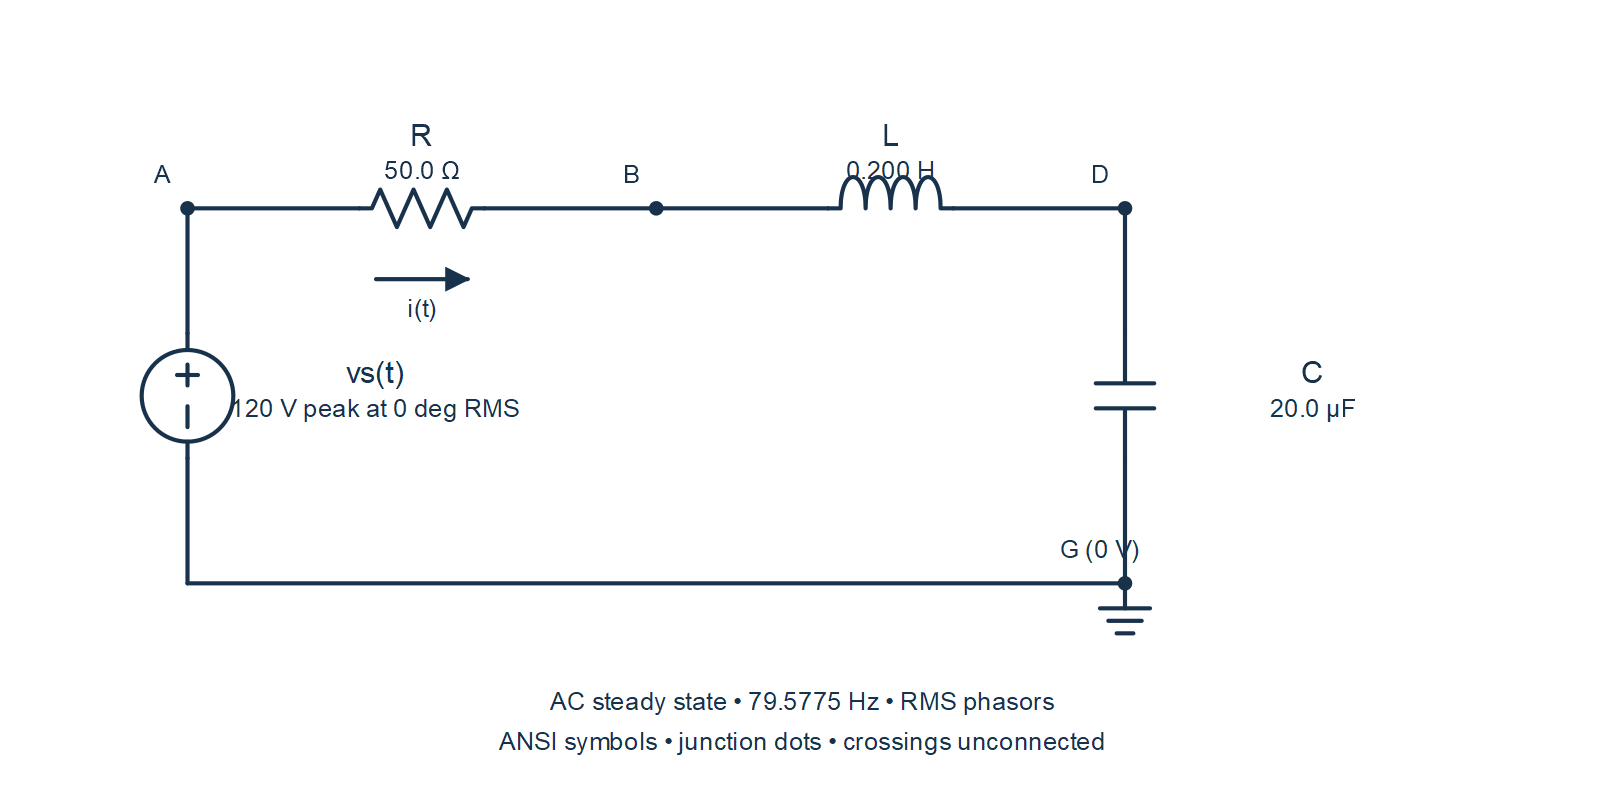
\includegraphics[width=0.82\linewidth]{day1_assets/s5-q3-ac-rlc.png}\end{center}

\begin{enumerate}
  \item \textbf{Resonant Frequency \& Resonance State ($\omega = \omega_0$) [4 points]:}
    \begin{enumerate}
      \item Calculate the resonant angular frequency $\omega_0 = \dfrac{1}{\sqrt{LC}}$ (in $\text{rad/s}$) and the corresponding linear frequency $f_0 = \dfrac{\omega_0}{2\pi}$ (in $\text{Hz}$).
      \item At $\omega = \omega_0$, compute $X_L(\omega_0)$, $X_C(\omega_0)$, the total impedance $Z(\omega_0)$, the peak current $I_0(\omega_0)$, the phase angle $\phi$, the time-averaged power $P_{\text{avg}} = \frac{1}{2}I_0^2 R$, and the peak voltages $V_{R,0}, V_{L,0}, V_{C,0}$. Explain how your values of $V_{L,0}$ and $V_{C,0}$ are consistent with KVL and $V_0 = 120\text{ V}$.
    \end{enumerate}
  
  \item \textbf{Low-Frequency Operation ($\omega_1 = 250\text{ rad/s}$) [4 points]:}
    \begin{enumerate}
      \item At $\omega_1 = 250\text{ rad/s}$, compute $X_L(\omega_1)$, $X_C(\omega_1)$, the net reactance $X(\omega_1) = X_L - X_C$, and the impedance $Z(\omega_1) = \sqrt{R^2 + (X_L - X_C)^2}$.
      \item Find the current amplitude $I_0(\omega_1)$, the phase angle $\phi_1 = \arctan\left(\dfrac{X_L - X_C}{R}\right)$ (in degrees), the power factor $\cos\phi_1$, the average power $P_{\text{avg}}(\omega_1)$, and write the steady-state current $i(t) = I_0\cos(\omega_1 t - \phi_1)$.
    \end{enumerate}
  
  \item \textbf{High-Frequency Operation ($\omega_2 = 1000\text{ rad/s}$) [4 points]:}
    \begin{enumerate}
      \item At $\omega_2 = 1000\text{ rad/s}$, compute $X_L(\omega_2)$, $X_C(\omega_2)$, $X(\omega_2) = X_L - X_C$, $Z(\omega_2)$, $I_0(\omega_2)$, $\phi_2$ (in degrees), and $P_{\text{avg}}(\omega_2)$.
      \item Compare your results at $\omega_1 = 250\text{ rad/s}$ and $\omega_2 = 1000\text{ rad/s}$: how do $Z$, $I_0$, $P_{\text{avg}}$, and the phase angle $\phi$ compare between these two frequencies, and why?
    \end{enumerate}
  
\end{enumerate}
\vspace{1.2in}


\newpage



\subsection*{04 $\cdot$ Frequency-Response Graphs \& Voltage Phasor Diagrams \hfill [Ch. 31 $\cdot$ 10 Points $\cdot$ 2 DRAW]}

For the series AC RLC circuit of Exercise 03 ($V_0 = 120\text{ V}, R = 50.0\ \Omega, L = 0.200\text{ H}, C = 20.0\ \mu\text{F}$):

\begin{enumerate}
  \item \textbf{Graph (i) --- Reactances \& Impedance vs. Angular Frequency [3 points]:} On the top-left grid below, plot $X_L(\omega) = \omega L$, $X_C(\omega) = \frac{1}{\omega C}$, and $Z(\omega) = \sqrt{R^2 + (X_L - X_C)^2}$ (\textbf{dependent variables}, vertical axis, in $\Omega$) vs. driving angular frequency $\omega$ (\textbf{independent variable}, horizontal axis, in $\text{rad/s}$) from $\omega = 0$ to $\omega = 1000\text{ rad/s}$. Label the coordinates of the reactance crossover point where $X_L(\omega_0) = X_C(\omega_0)$ and the minimum impedance point $(\omega_0, Z_{\min})$.
  \item \textbf{Graph (ii) --- Resonance Current Curve for Low $R$ vs. High $R$ [3 points]:} On the top-right grid below, plot the current amplitude $I_0(\omega) = \frac{V_0}{Z(\omega)}$ (\textbf{dependent variable}, vertical axis, in $\text{A}$) vs. driving angular frequency $\omega$ (\textbf{independent variable}, horizontal axis, in $\text{rad/s}$) for (1) $R = 50.0\ \Omega$ and (2) $R = 120\ \Omega$. Label the resonant frequency $\omega_0$ and the peak current $I_{0,\max}$ for each curve.
  \item \textbf{Diagrams (iii) \& (iv) --- Voltage Phasor Diagrams [4 points]:} On the bottom axes (where the current phasor $\vec{I}_0$ lies along the $+x$ reference axis at $0^\circ$), draw to scale the individual voltage phasors $\vec{V}_R$, $\vec{V}_L$, $\vec{V}_C$, the net reactive phasor $\vec{V}_L + \vec{V}_C$, and the resultant source phasor $\vec{V}_s = \vec{V}_R + (\vec{V}_L + \vec{V}_C)$, and label the phase angle $\phi$ and whether the circuit is capacitive or inductive for:
    \begin{itemize}
      \item \textbf{(iii) $\omega_1 = 250\text{ rad/s}$} (using your values from Exercise 03b).
      \item \textbf{(iv) $\omega_2 = 1000\text{ rad/s}$} (using your values from Exercise 03c).
    \end{itemize}
  
\end{enumerate}

\begin{center}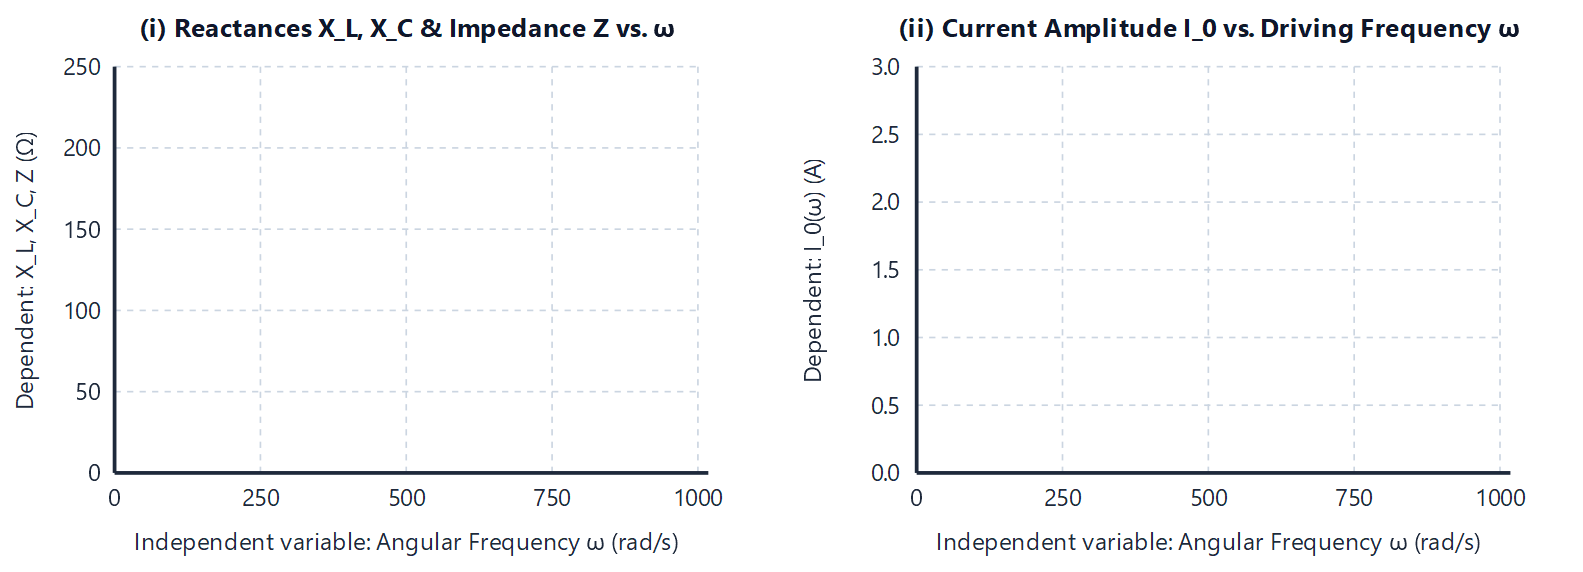
\includegraphics[width=0.82\linewidth]{day1_assets/s5-q4-grid-blank.png}\end{center}
\begin{center}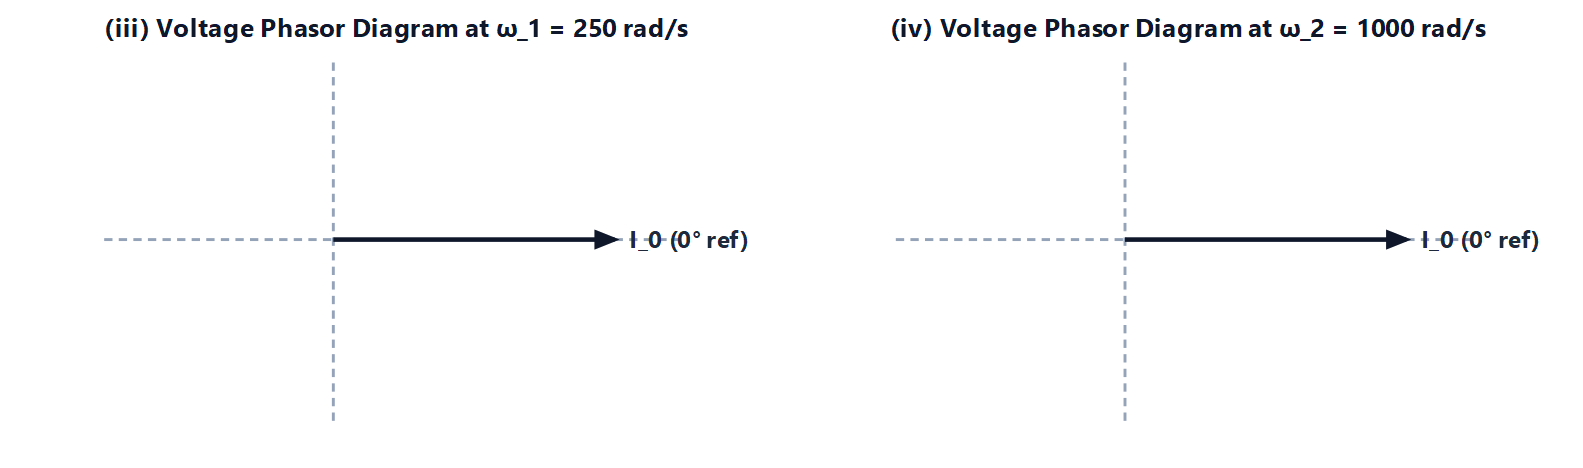
\includegraphics[width=0.82\linewidth]{day1_assets/s5-q4-phasors-blank.png}\end{center}

\end{document}
